\documentclass{beamer}

%\includeonlyframes{current}

\usepackage[T1]{fontenc}
\usepackage[utf8]{inputenc}
\usepackage{unicode}
\usepackage[american]{babel}
\usepackage{amsmath,amssymb,amsthm}
\usepackage[nosfdefault]{comicneue}
\usepackage[normalem]{ulem}
\usepackage{tikz}
\usepackage{tikzsymbols}
\usetikzlibrary{arrows,matrix,decorations,decorations.text,decorations.pathmorphing,calc,positioning}
\usepackage[backend=biber,citestyle=authoryear-comp,bibstyle=beamer,doi=false,isbn=false,url=true,maxnames=10]{biblatex}
\bibliography{defeo}

\mode<presentation>{%
  \usetheme{Boadilla}
}
\beamertemplatenavigationsymbolsempty
\setbeamercolor*{title}{fg=blue!50!black}
\setbeamercolor*{titlegraphic}{fg=blue!20!black}

\usepackage{sourcesanspro}
\usepackage[amssymb,amsfonts]{concmath}
\usefonttheme[onlymath]{serif}

\renewcommand{\emph}[1]{{\usebeamercolor[fg]{structure}#1}}

%\let\footcite\footnote

\newcommand{\C}{ℂ}
\newcommand{\R}{ℝ}
\newcommand{\Z}{ℤ}
\newcommand{\N}{ℕ}
\newcommand{\Q}{ℚ}
\newcommand{\F}{\mathbb{F}}
\renewcommand{\P}{\mathbb{P}}
\renewcommand{\O}{\mathcal{O}}
\newcommand{\tildO}{\mathcal{\tilde{O}}}
\newcommand{\poly}{\operatorname{poly}}
\newcommand{\polylog}{\operatorname{polylog}}
\newcommand{\End}{\operatorname{End}}
\newcommand{\Hom}{\operatorname{Hom}}
\newcommand{\Gal}{\operatorname{Gal}}
\newcommand{\chr}{\operatorname{char}}
\newcommand{\Cl}{\operatorname{Cl}}
\newcommand{\GL}{\operatorname{GL}}
\renewcommand{\a}{{\mathfrak{a}}}
\renewcommand{\b}{{\mathfrak{b}}}
\newcommand{\cyc}[1]{{〈 #1 〉}}
\newcommand{\ord}{\operatorname{ord}}
\newcommand{\mat}[1]{\left(\begin{smallmatrix}#1\end{smallmatrix}\right)}

\pgfkeys{/triangle/.code=\tikzset{x={(-0.5cm,-0.866cm)},y={(1cm,0cm)}}}
\pgfkeys{/lattice/.code n args={4}{\tikzset{cm={#1,#2,#3,#4,(0,0)}}}}

\newcommand{\axes}[4]{
  \clip (#1,#3) rectangle (#2,#4);
  \draw [thin, gray, -latex] (#1,0) -- (#2,0);% Draw x axis
  \draw [thin, gray, -latex] (0,#3) -- (0,#4);% Draw y axis
}

\newcommand{\lattice}[2]{
  \draw[style=help lines,dashed] (#1-1,#1-1) grid[step=1] (#2+1,#2+1);
  \foreach \x in {#1,...,#2}{
    \foreach \y in {#1,...,#2}{
      \node[draw,circle,inner sep=2pt,fill] at (\x,\y) {};
      % Places a dot at those points
    }
  }
}

\newcommand{\bl}[1]{\textcolor{blue}{#1}}
\newcommand{\rd}[1]{\textcolor{red}{#1}}
\newcommand{\gr}[1]{\textcolor{green}{#1}}

% This command defines a triangle of dots of given height
\newcommand{\dottriangle}[2][\i-\j]{%
  \foreach \i in {0,...,#2} {%
    \foreach \j in {0,...,\i} {%
      \draw(\i,\j) node{#1};%
    }%
  }}


\title{Isogeny graphs in cryptography}
\author[Luca De Feo]{Luca De Feo}
\date[Mar 18, 2019 --- Maths of PKC]{March 18, 2019\\
  \href{https://mathsofpkc.sciencesconf.org/}{Mathematical foundations of asymmetric cryptography}\\
  Aussois, Savoie
}
\institute[U Paris Saclay]{Université Paris Saclay, UVSQ}

\begin{document}

\frame[plain]{
  \begin{tikzpicture}[remember picture,overlay]
    \node[at=(current page.center), opacity=0.7] {
      \includegraphics[width=1.2\paperwidth]{aussois.jpg}
    };
  \end{tikzpicture}
  \vspace{-1.1cm}
  \usebeamercolor[fg]{titlegraphic}
  {\bf \titlepage}
  \vspace{0.5cm}
  \begin{center}
    \textcolor{white}{Slides online at}~~~\href{https://defeo.lu/docet/}{https://defeo.lu/docet/}
  \end{center}
}

%% 

\begin{frame}
  \frametitle{Overview}
  \tableofcontents  
\end{frame}

%%
%% 

\section{Isogeny graphs}

\subsection{Elliptic Curves}

\begin{frame}{Elliptic curves}
  \begin{columns}
    \begin{column}{0.4\textwidth}
      Let $k$ be a field of characteristic $\ne 2,3$.

      An \emph{elliptic curve \textit{defined over $k$}} is the locus
      in the \emph{projective space} $\P^2(\bar{k})$ of an equation
      \[\emph{Y^2Z = X^3 + aXZ^2 + bZ^3},\]
      where $a,b\in k$ and $4a^3+27b^2\ne 0$.

      \begin{itemize}
      \item<2-> $\O=(0:1:0)$ is the \emph{point at infinity};
      \item<3-> $y^2 = x^3 + ax + b$ is the \emph{affine Weierstrass equation}.
      \end{itemize}
    \end{column}
    \begin{column}{0.6\textwidth}
      \begin{center}
        \begin{tikzpicture}[domain=-2.4566:4,samples=100,yscale=1/2]
          \draw plot (\x,{sqrt(\x*\x*\x-4*\x+5)});
          \draw plot (\x,{-sqrt(\x*\x*\x-4*\x+5)});

          \draw[thin,gray,-latex] (0,-7) -- (0,7);
          \draw[thin,gray,-latex] (-3,0) -- (4,0);
        \end{tikzpicture}
      \end{center}
    \end{column}
  \end{columns}
\end{frame}

%%

\begin{frame}{The group law}
  \begin{columns}
    \begin{column}{0.4\textwidth}
      \begin{block}{Bezout's theorem}
        Every line cuts $E$ in exactly three points (counted with
        multiplicity).
      \end{block}

      Define a \emph{group law} such that any three colinear points
      add up to zero.

      \begin{itemize}
      \item<2-> The law is \emph{algebraic}\\ (it has \textit{formulas});
      \item<3-> The law is \emph{commutative};
      \item<3-> $\O$ is the \emph{group identity};
      \item<3-> \emph{Opposite points} have the same $x$-value.
      \end{itemize}
    \end{column}
    \begin{column}{0.6\textwidth}
      \begin{center}
        \begin{tikzpicture}[domain=-2.4566:4,samples=100,yscale=1/2]
          \draw plot (\x,{sqrt(\x*\x*\x-4*\x+5)});
          \draw plot (\x,{-sqrt(\x*\x*\x-4*\x+5)});

          \draw[thin,gray,-latex] (0,-7) -- (0,7);
          \draw[thin,gray,-latex] (-3,0) -- (4,0);
          \draw (-3,1) -- (4,8/3+3);
          \begin{scope}[every node/.style={draw,circle,inner sep=1pt,fill},cm={1,2/3,0,0,(0,3)}]
            \node at (-2.287980,0) {};
            \node at (-0.535051,0) {};
            \node at (3.267475,0) {};
          \end{scope}
          \begin{scope}[every node/.style={yshift=0.3cm},cm={1,2/3,0,0,(0,3)}]
            \node at (-2.287980,0) {$P$};
            \node at (-0.535051,0) {$Q$};
            \node at (3.267475,0) {$R$};
          \end{scope}

          \draw[dashed] (3.267475,3.267475*2/3+3) -- (3.267475,-3.267475*2/3-3) 
          node[draw,circle,inner sep=1pt,fill] {}
          node[xshift=-0.1cm,anchor=east] {$P+Q$};
        \end{tikzpicture}
      \end{center}
    \end{column}
  \end{columns}
\end{frame}

%%

\begin{frame}{Why should I care? (Diffie--Hellman key exchange)}
  \begin{description}
  \item[Goal:] Alice and Bob have never met before. They are chatting
    over a public channel, and want to agree on a \emph{shared secret}
    to start a private conversation.
  \item[Setup:] They agree on a (large) cyclic group $G=〈g〉$
    of (prime) order $q$.
  \end{description}

  \begin{center}
    \begin{tikzpicture}
      \node at (0,0) {\bf Alice};
      \node at (7,0) {\bf Bob};
      \node at (0,-1) {pick random \alert{$a∈ℤ/qℤ$}};
      \node at (0,-1.5) {compute $A=g^a$};
      \node at (7,-1) {pick random \alert{$b∈ℤ/qℤ$}};
      \node at (7,-1.5) {compute $B=g^b$};
      \draw[->]
      (1,-2) to node[auto] {$A$} (6,-2);
      \draw[->] (6,-2.5) to node[auto] {$B$} (1,-2.5);
      \node at (3.5,-3.5) {\emph{Shared secret} is \alert{$B^a=g^{ab}=A^b$}};
    \end{tikzpicture}
  \end{center}
\end{frame}

%%

\begin{frame}{Brief history of DH key exchange}
  \begin{description}
  \item[1976] Diffie \& Hellman publish \emph{New directions in
      cryptography}, suggest using $G=\F_p^\ast$.
  \item[1978] Pollard publishes his \emph{discrete logarithm}
    algorithm ($O(\sqrt{\# G})$ complexity).
  \item[1980] Miller and Koblitz independently suggest using
    \emph{elliptic curves} $G=E(\F_p)$.
  \item[1994] Shor publishes his quantum polynomial time
    \emph{discrete logarithm / factoring} algorithm.
  \item[2005] NSA standardizes elliptic curve key agreement (ECDH) and
    signatures ECDSA.
  \item[2017] $\sim 70\%$ of web traffic is secured by ECDH and/or
    ECDSA.
  \item[2017] NIST launches \emph{post-quantum competition}, says
    ``not to bother moving to elliptic curves, if you haven't yet''.
  \end{description}
\end{frame}

%% 

\begin{frame}{Why should I care? (cont'd)}

  {\large\emph{But, also:}}
  \begin{itemize}
  \item Elliptic Curve Factoring Method (Lenstra '85);
  \item Elliptic Curve Primality Proving (Atkin, Morain '86-'93);
  \item Efficient normal bases for finite fields (Couveignes, Lercier '10);
  \item \dots
  \end{itemize}
\end{frame}

%%

\begin{frame}{What are elliptic curves?}
  \begin{block}{For mathematicians}
    \begin{itemize}
    \item The \emph{smooth projective curves of genus 1} (with a
      distinguished point);
    \item The simplest \emph{abelian varieties} (dimension 1);
    \item Finitely generated abelian groups of mysterious free rank
      (aka \emph{BSD conjecture});
    \item What you use to make examples.
    \end{itemize}
  \end{block}

  \pause
  
  \begin{block}{For cryptographers}
    \begin{itemize}
    \item \emph{Finite abelian} groups (often cyclic);
    \item Easy to compute the order;
    \item ``2-dimensional'' generalizations of $μ_k$ (the \emph{roots
        of unity} of $k$)\dots
    \item \dots with \emph{bilinear maps} (aka \emph{pairings})!
    \end{itemize}
  \end{block}
\end{frame}

%%

\begin{frame}{Isomorphisms}
  \begin{block}{Isomorphisms}
    The only \emph{invertible algebraic maps} between elliptic curves
    are of the form
    \[(x,y) \mapsto (u^2x, u^3y)\]
    for some $u\in\bar{k}$.

    They are \emph{group isomorphisms}.
  \end{block}

  \begin{block}{$j$-Invariant}
    Let $E\;:\;y^2=x^3+ax+b$, its \emph{$j$-invariant} is
    \[j(E) = 1728\frac{4a^3}{4a^3+27b^2}.\]

    Two elliptic curves $E,E'$ are \emph{isomorphic} if and only if
    $j(E)=j(E')$.
  \end{block}
\end{frame}

%%

\begin{frame}{Group structure}
  \begin{block}{Torsion structure}
    Let $E$ be defined over an algebraically closed field $\bar{k}$ of
    characteristic $p$.
    \begin{align*}
      E[m] \simeq\quad& \Z/m\Z\times\Z/m\Z  &\text{if $p\nmid m$,}\\[1em]
                 &\Z/p^e\Z & \text{\emph{ordinary} case,}\\[-1.7em]
      E[p^e] \simeq\Biggl\{& \\[-1.7em]
                 &\{\O\} & \text{\emph{supersingular} case.}
    \end{align*}
  \end{block}

  \begin{block}{Finite fields (Hasse's theorem)}
    Let \emph{$E$} be defined over a finite field \emph{$\F_q$}, then
    \[\lvert\#E(\F_q) - q - 1\rvert \le 2\sqrt{q}.\]
    In particular, there exist integers \emph{$n_1$} and
    \emph{$n_2|\gcd(n_1,q-1)$} such that
    \[E(\F_q) ≃ ℤ/n_1ℤ × ℤ/n_2ℤ.\]
  \end{block}
\end{frame}


%%%%%%%%%%%%%%%%%%%%%%%%%%%%%%%%%%%%%%%
%%%%%%%%%%%%%%%%%%%%%%%%%%%%%%%%%%%%%%%

\subsection{Isogenies}

\begin{frame}{What is \alt<2->{\xout{scalar multiplication} an
      isogeny}{scalar multiplication}?}

  \begin{overlayarea}{\textwidth}{4em}
    \Large
    \[
      \alt<3->{ϕ}{[n]}
      \;:\; P \mapsto
      \alt<3->{ϕ(P)}{\underbrace{P + P + \cdots + P}_{n\text{ times}}}\]
  \end{overlayarea}
  
  \begin{itemize}
  \item A map \emph{$E\to \alt<4->{\xout{E} E'}{E\phantom{\xout{}}}$},
  \item a \emph{group morphism},
  \item with \emph{finite kernel}\\
    \alt<5->{(\xout{the torsion group $E[n]≃(ℤ/nℤ)^2$} any
      finite subgroup \emph{$H\subset E$})}{(the torsion group
      \emph{$E[n]\simeq(ℤ/nℤ)^2$})},
  \item \emph{surjective} (in the algebraic closure),
  \item given by \emph{rational maps} of degree \alt<6->{\xout{$n^2$}
      \emph{$\#H$}}{\emph{$n^2$}}.
  \end{itemize}

  \begin{uncoverenv}<7->
    (Separable) isogenies $⇔$ finite subgroups:
    \alert{\[0 → H → E \overset{ϕ}{→} E' \to 0\]}
    The kernel \emph{$H$} determines the image curve \emph{$E'$} up to
    isomorphism \[\emph{E/H\overset{\text{\tiny def}}{=}E'}.\]
  \end{uncoverenv}
\end{frame}

%%

\begin{frame}{Isogenies: an example over $\F_{11}$}
  \begin{tikzpicture}[scale=0.4]
    \begin{scope}
      \node[anchor=center] at (0,7) {$E \;:\; y^2 = x^3 + x$};

      \uncover<-1>{
        \draw[thin,gray] (0,-6) -- (0,6);
        \draw[thin,gray] (-6,0) -- (6,0);
      }

      \foreach \x/\y in {0/0,5/3,-4/3,-3/5,-2/1,-1/3} {
        \draw[blue,fill] (\x,\y) circle (0.2) node(E_\x_\y){}
        (\x,-\y) circle (0.2) node(E_\x_-\y){};
      }

      \uncover<2->{\draw[red,fill] (0,0) circle (0.3);}
    \end{scope}

    \draw[black!10!white,thick] (8,-7) -- +(0,14);
    
    \begin{scope}[shift={(16,0)}]
      \node at (0,7) {$E' \;:\; y^2 = x^3 - 4x$};

      \uncover<-1>{
        \draw[thin,gray] (0,-6) -- (0,6);
        \draw[thin,gray] (-6,0) -- (6,0);
      }

      \foreach \x/\y in {0/0,2/0,3/2,4/2,6/4,-2/0,-1/5} {
        \draw[color=blue,fill] (\x,\y) circle (0.2) node(F_\x_\y){}
        (\x,-\y) circle (0.2) node(F_\x_-\y){};
      }
    \end{scope}

    \begin{scope}[color=red,-latex,dashed]
      \begin{uncoverenv}<2->
        \path
        (E_5_3) edge (F_3_2)
        (E_-4_3) edge (F_4_-2)
        (E_-3_5) edge (F_4_2)
        (E_-2_1) edge (F_3_-2)
        (E_-1_3) edge (F_-2_0);
      \end{uncoverenv}
      \begin{uncoverenv}<2->
        \path
        (E_5_-3) edge (F_3_-2)
        (E_-4_-3) edge (F_4_2)
        (E_-3_-5) edge (F_4_-2)
        (E_-2_-1) edge (F_3_2)
        (E_-1_-3) edge (F_-2_0);
      \end{uncoverenv}
    \end{scope}
  \end{tikzpicture}
  
  \begin{columns}
    \begin{column}{0.5\textwidth}
      \[ϕ(x,y) = \left(\frac{x^2 + 1}{x},\quad y\frac{x^2-1}{x^2}\right)\]
    \end{column}
    \begin{column}{0.5\textwidth}
      \begin{itemize}
      \item<2-> Kernel generator in \alert{red}.
      \item<2-> This is a degree $2$ map.
      \item<2-> Analogous to $x↦x^2$ in $\F_q^*$.
      \end{itemize}
    \end{column}
  \end{columns}
\end{frame}

%%

\begin{frame}{Isogeny properties}
  Let $\phi:E\to E'$ be an isogeny defined over a field $k$ of
  characteristic $p$.
  
  \begin{itemize}
  \item $k(E)$ is the \emph{field of all rational functions} from $E$
    to $k$;
  \item $\phi^\ast k(E')$ is the subfield of $k(E)$ defined as
    \[\phi^\ast k(E') = \{ f\circ\phi \;\vert\; f\in k(E') \}.\]
  \end{itemize}

  \begin{block}{Degree, separability}
    \begin{enumerate}
    \item The \emph{degree} of $\phi$ is 
      $\deg\phi = [k(E):\phi^\ast k(E')]$. It is always finite.
    \item $\phi$ is said to be \emph{separable}, \emph{inseparable}, or
      \emph{purely inseparable} if the extension of function fields is.
    \item \alert<2>{If $\phi$ is separable, then
        $\deg\phi = \#\ker\phi$.}
    \item If $\phi$ is purely inseparable, then $\ker\phi=\{\O\}$ and
      $\deg\phi$ is a power of $p$.
    \item Any isogeny can be decomposed as a product of a separable and
      a purely inseparable isogeny.
    \end{enumerate}
  \end{block}
\end{frame}

%%

\begin{frame}{The dual isogeny}
  Let $\phi:E\to E'$ be an isogeny of degree $m$. 
  There is a unique isogeny $\hat{\phi}:E'\to E$ such that
  \[\hat{\phi}\circ\phi = [m]_E, \quad \phi\circ\hat{\phi} = [m]_{E'}.\]
  $\hat{\phi}$ is called the \emph{dual isogeny of $\phi$}; it has the
  following properties:
  
  \begin{enumerate}
  \item $\hat{\phi}$ is defined over $k$ if and only if $\phi$ is;
  \item $\widehat{\psi\circ\phi} = \hat{\phi}\circ\hat{\psi}$ for any isogeny $\psi:E'\to E''$;
  \item $\widehat{\psi+\phi} = \hat{\psi} + \hat{\phi}$ for any isogeny $\psi:E\to E'$;
  \item $\deg \phi = \deg\hat{\phi}$;
  \item $\hat{\hat{\phi}} = \phi$.
  \end{enumerate}
\end{frame}


%%%%%%%%%%%%%%%%%%%%%%%%%%%%%%%%%%%%%%%
%%%%%%%%%%%%%%%%%%%%%%%%%%%%%%%%%%%%%%%

\subsection{Isogeny graphs}

\begin{frame}
  \frametitle{Isogeny graphs}
  
  \vspace{-2mm}

  \begin{columns}
    \begin{column}{0.65\textwidth}
      We look at the graph of elliptic curves with isogenies \emph{up
        to isomorphism}.  We say two \alert{isogenies} $ϕ,ϕ'$
      are \alert{isomorphic} if:
    \end{column}
    \begin{column}{0.3\textwidth}
      \begin{center}
        \begin{tikzpicture}[node distance=4em]
          \node(E){$E$}; 
          \node(E1)[right of=E]{$E'$};
          \node(E2)[below of=E1]{$E'$};
          \scriptsize
          \path[->] (E) edge node[auto]{$ϕ$} (E1);
          \path[->] (E) edge node[auto,swap]{$ϕ'$} (E2);
          \path[<->] (E1) edge node[rotate=270] {\large$\widetilde{}$} (E2);
        \end{tikzpicture}
      \end{center}
    \end{column}
  \end{columns}

  \emph{Example:} Finite field, ordinary case, graph of isogenies of degree $3$.

  \begin{center}
    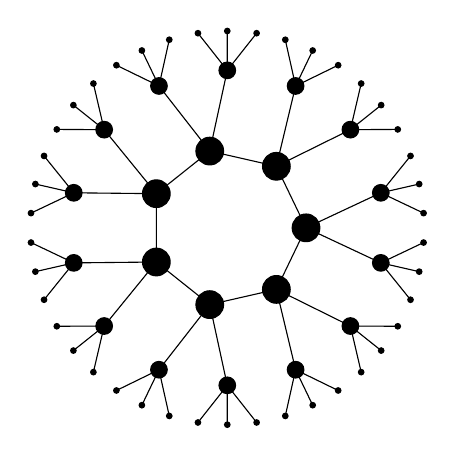
\begin{tikzpicture}[]
      \begin{scope}
        \def\crater{7}
        \foreach \i in {1,...,\crater} {
          \draw[fill] (360/\crater*\i:1cm) circle (5pt);
          \draw (360/\crater*\i : 1cm) -- (360/\crater*\i+360/\crater : 1cm);
          \foreach \j in {-1,1} {
            \draw[fill] (360/\crater*\i : 1cm) -- (360/\crater*\i + \j*360/\crater/4 : 2cm) circle (3pt);
            \foreach \k in {-1,0,1} {
              \draw[fill] (360/\crater*\i + \j*360/\crater/4 : 2cm) --
              (360/\crater*\i + + \j*360/\crater/4 + \k*360/\crater/6 : 2.5cm) circle (1pt);
            }
          }
        }
      \end{scope}
    \end{tikzpicture}
  \end{center}
\end{frame}

%%

\begin{frame}{What do isogeny graphs look like?}
  \begin{columns}
    \begin{column}{0.46\textwidth}
      \begin{block}{Torsion subgroups ($ℓ$ prime)}
        In an algebraically closed field:
        \[\emph{E[ℓ] = 〈P,Q〉 ≃ (ℤ/ℓℤ)^2}\]
        \[\Downarrow\]
        There are exactly \emph{$ℓ+1$} cyclic subgroups \emph{$H⊂E$}
        of order $ℓ$:
        \[\emph{〈P+Q〉, 〈P+2Q〉, \dots, 〈P〉, 〈Q〉}\]
        \[\Downarrow\]
        There are exactly \emph{$ℓ+1$} distinct isogenies of degree
        \emph{$ℓ$}.
      \end{block}
    \end{column}
    \begin{column}{0.54\textwidth}
      \centering
      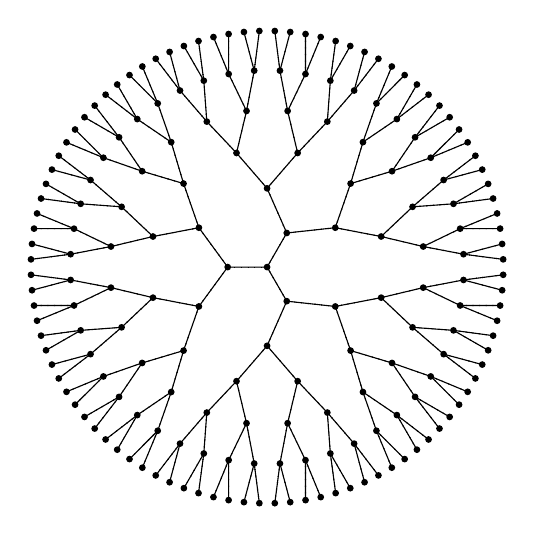
\begin{tikzpicture}[scale=0.5]
        \def\levels{6}
        \draw[fill] (0:0) circle (2pt);
        \foreach \i in {1,...,\levels} {
          \pgfmathparse{3*2^\i}
          \let\nodes\pgfmathresult
          \foreach \j in {1,3,...,\nodes} {
            \pgfmathparse{\j + (-1)^div(\j,2)}
            \let\lower\pgfmathresult
            \ifthenelse{\i = \levels}{
              \draw[dotted] (360/\nodes*\j : \i) --
              (360/\nodes*\lower : \i - 1);
            }{
              \draw[fill] (360/\nodes*\j : \i) circle (2pt) --
              (360/\nodes*\lower : \i - 1);
            }
          }
        }
      \end{tikzpicture}
      (non-CM) $2$-isogeny graph over $ℂ$
    \end{column}
  \end{columns}
\end{frame}  
  
%%

\begin{frame}{What happens over a finite field $\F_p$?}
  \begin{block}{Rational isogenies ($ℓ≠p$)}
    In the algebraic closure \emph{$\bar{\F}_p$}
    \[\emph{E[ℓ] = 〈P,Q〉 ≃ (ℤ/ℓℤ)^2}\]
    However, an isogeny is \emph{defined over $\F_p$} only if its kernel
    is \emph{Galois invariant}.
  \end{block}

  \begin{columns}
    \begin{column}{0.47\textwidth}
      Enter the \emph{Frobenius map}
      \begin{align*}
        π : E &→ E\\
        (x,y) &↦ (x^p,y^p)
      \end{align*}
      \emph{$E$} is seen here as a curve over \emph{$\bar{\F}_p$}.
    \end{column}
    \begin{column}{0.47\textwidth}
      \begin{block}{The Frobenius action on $E[ℓ]$}
        \animate<2-5>
        \transdissolve<2-5>
        \begin{tikzpicture}[]
          \uncover<1>{
            \node at (0,0){$π(P) =$};   
            \node at (0,-0.7){$π(Q) =$};
          }
          \node at (1.8,0){$a\uncover<-3>{P +} b\uncover<-3>{Q}$};
          \node at (1.8,-0.7){$c\uncover<-3>{P +} d\uncover<-3>{Q}$};
          \uncover<3->{
            \node at (0.8,-0.35){$\Biggl($}; \node at (2.7,-0.35){$\Biggr)$};
          }
          \uncover<5->{
            \node at (0.3,-0.35){$π:$};
            \node at (3.3,-0.35){$\mod ℓ$};
          }
        \end{tikzpicture}

        \uncover<6->{We identify \emph{$π|E[ℓ]$} to a conjugacy class
          in \emph{$\GL(ℤ/ℓℤ)$}.}
      \end{block}
    \end{column}
  \end{columns}
\end{frame}

%%

\begin{frame}{What happens over a finite field $\F_p$?}
  \begin{center}
    Galois invariant subgroups of \emph{$E[ℓ]$}\\
    =\\
    eigenspaces of \emph{$π∈\GL(ℤ/ℓℤ)$}\\
    =\\
    rational isogenies of \emph{degree $ℓ$}
  \end{center}
  \pause
  \begin{block}{How many Galois invariant subgroups?}
    \begin{itemize}
    \item \emph{$π|E[ℓ] \sim \mat{λ&0\\0&λ}$}
      \hfill $→ \emph{ℓ+1}$ isogenies
    \item \emph{$π|E[ℓ] \sim \mat{λ&0\\0&μ}$} with \emph{$λ≠μ$}
      \hfill $→$ \emph{two} isogenies
    \item \emph{$π|E[ℓ] \sim \mat{λ&*\\0&λ}$}
      \hfill $→$ \emph{one} isogeny
    \item \emph{$π|E[ℓ]$} is not diagonalizable over \emph{$ℤ/ℓℤ$}
      \hfill $→$ \emph{no} isogeny
    \end{itemize}
  \end{block}
\end{frame}

%%

\begin{frame}{Weil pairing}
  Let $(N,p)=1$, fix any basis \emph{$E[N]=〈R,S〉$}. For any points
  \emph{$P,Q∈E[N]$}
  \begin{align*}
    P &= aR + bS\\
    Q &= cR + dS
  \end{align*}
  the form \emph{$\det_N(P,Q) = \det\mat{a&b\\c&d} = ad - bc ∈ ℤ/Nℤ$}\\
  is \emph{bilinear}, non-degenerate, and independent from the choice
  of basis.

  \begin{block}{Theorem}
    Let $E/\F_q$ be a curve, there exists a Galois invariant bilinear
    map
    \[e_N: E[N] × E[N] → μ_N ⊂ \bar\F_q,\] \\
    called the \emph{Weil pairing of order $N$}, and a primitive
    $N$-th root of unity \emph{$ζ∈\bar\F_q$} such that
    \[e_N(P,Q) = ζ^{\det_N(P,Q)}.\] \\
    The degree \emph{$k$} of the smallest extension such that
    \emph{$ζ∈\F_{q^k}$} is called the \emph{embedding degree} of the
    pairing.
  \end{block}
\end{frame}

%%

\begin{frame}{Weil pairing and isogenies}
  \begin{block}{Note}
    The Weil pairing is Galois invariant $\;\;⇔\;\;\emph{\det(π|E[N]) = q}$.
  \end{block}

  \begin{block}{Theorem}
    Let \emph{$ϕ:E→E'$} be an isogeny and \emph{$\hat{ϕ}:E'→E$} its dual. \\
    Let \emph{$e_N$} be the Weil pairing of $E$ and \emph{$e_N'$} that
    of $E'$. %
    Then, for
    \[e_N(P,\hat{ϕ}(Q)) = e_N'(ϕ(P),Q),\]
    for any \emph{$P∈E[N]$} and \emph{$Q∈E'[N]$}.
  \end{block}
  
  \begin{block}{Corollary}
    \[e_N'(ϕ(P),ϕ(Q)) = e_N(P,Q)^{\deg ϕ}.\]
  \end{block}
\end{frame}

%%%%%%%%%%%%%%%%%%%%%%%%%%%%%%%%%%%%%%%
%%%%%%%%%%%%%%%%%%%%%%%%%%%%%%%%%%%%%%%

\subsection{Endomorphism rings}

\begin{frame}{From local to global}
  \begin{block}{Theorem (Hasse)}
    Let $E$ be defined over a finite field $\F_q$. Its Frobenius map
    $π$ satisfies a quadratic equation
    \[π^2 - tπ + q = 0\] %
    for some \emph{$|t|\le2\sqrt{q}$}, called the \emph{trace}
    of $π$.  The trace $t$ is coprime to $q$ if and only if $E$ is
    ordinary.
  \end{block}
  
  \begin{block}{Endomorphisms}
    An isogeny $E→E$ is also called an \emph{endomorphism}. Examples:
    \begin{itemize}
    \item scalar multiplication \emph{$[n]$},
    \item Frobenius map \emph{$π$}.
    \end{itemize}
    With \emph{addition} and \emph{composition}, the endomorphisms
    form a ring \emph{$\End(E)$}.
  \end{block}
\end{frame}

%%

\begin{frame}{The endomorphism ring}

  \begin{block}{Theorem (Deuring)}
    Let $E$ be an \emph{ordinary} elliptic curve defined over a finite
    field $\F_q$.\\
    Let $π$ be its Frobenius endomorphism, and $D_π=t^2-4q<0$ the
    \emph{discriminant} of its minimal polynomial.

    Then $\End(E)$ is isomorphic to an \emph{order} $\O$ of the
    \emph{quadratic imaginary field} $ℚ(\sqrt{D_π})$.%
    \footnote{An order is a subring that is a $ℤ$-module of rank $2$
      (equiv., a $2$-dimensional $ℝ$-lattice).}
  \end{block}

  In this case, we say that $E$ has \emph{complex multiplication} (CM)
  by $\O$.

  \begin{block}{Theorem (Serre-Tate)}
    CM elliptic curves $E,E'$ are isogenous iff
    \emph{$\End(E)⊗ℚ≃\End(E')⊗ℚ$}.

    \medskip
    
    \textbf{\emph{Corollary:}} $E/\F_p$ and $E'/\F_p$ are isogenous
    over $\F_p$ iff \emph{$\#E(\F_p)=\#E'(\F_p)$}.
  \end{block}

\end{frame}

%%

\begin{frame}{Endomorphism rings of ordinary curves}
  \begin{block}{Classifying quadratic orders}
    Let $K$ be a quadratic number field, and let $\O_K$ be its ring of
    integers.
    \begin{itemize}
    \item Any order $\O\subset K$ can be written as $\O=\Z+f\O_K$ for
      an integer $f$, called the \emph{conductor} of $\O$, denoted by
      $[\O_K:\O]$.
    \item If $D_K$ is the \emph{discriminant} of $K$, the discriminant
      of $\O$ is $f^2D_K$.
    \item If $\O,\O'$ are two orders with discriminants $D,D'$, then
      \emph{$\O\subset\O'$ iff $D'|D$}.
    \end{itemize}
  \end{block}

  \medskip
  
  \centering
  \begin{tikzpicture}[xscale=3,yscale=1.1]
    \node(OK) at (0,0) {$\O_K$};
    \node(O2) at (-1,-1) {$\Z+2\O_K$};
    \node(O3) at (0,-1) {$\Z+3\O_K$};
    \node(O5) at (1,-1) {$\Z+5\O_K$};
    \node(O6) at (-1,-2) {$\Z+6\O_K$};
    \node(O10) at (0,-2) {$\Z+10\O_K$};
    \node(O15) at (1,-2) {$\Z+15\O_K$};
    \node(O30) at (0,-3) {$\Z[\pi]\simeq\Z+30\O_K$};

    \begin{scope}
      \draw
      (OK) edge (O2) edge (O3) edge (O5)
      (O2) edge (O6) edge (O10)
      (O3) edge (O6) edge (O15)
      (O5) edge (O10) edge (O15)
      (O30) edge (O6) edge (O15) edge (O10);
    \end{scope}
  \end{tikzpicture}
\end{frame}

%%%%%%%%%%%%%%%%%%%%%%%%%%%%%%%%%%%%%%%
%%%%%%%%%%%%%%%%%%%%%%%%%%%%%%%%%%%%%%%

\subsection{Ordinary graphs}

\begin{frame}{Volcanology \parencite{kohel}}

  \begin{columns}
    \begin{column}{0.5\textwidth}
      Let \emph{$E,E'$} be curves with respective endomorphism rings \emph{$\O,\O'⊂K$}.\\
      Let \emph{$ϕ:E→E'$} be an isogeny of prime degree \emph{$ℓ$},
      then:
    \end{column}
    \begin{column}{0.5\textwidth}
      \centering{}
      \begin{tabular}{l l}
        if $\O=\O'$, & $ϕ$ is \emph{horizontal};\\
        if $[\O':\O]=ℓ$, & $ϕ$ is \emph{ascending};\\
        if $[\O:\O']=ℓ$, & $ϕ$ is \emph{descending}.
      \end{tabular}      
    \end{column}
  \end{columns}

  \bigskip

  \centering
  \begin{tikzpicture}
    \def\crater{7}
    \foreach \i in {1,...,\crater} {
      \draw[fill] (360/\crater*\i:1cm) circle (5pt);
      \draw (360/\crater*\i : 1cm) -- (360/\crater*\i+360/\crater : 1cm);
      \foreach \j in {-1,1} {
        \draw[fill] (360/\crater*\i : 1cm) -- (360/\crater*\i + \j*360/\crater/4 : 2cm) circle (3pt);
        \foreach \k in {-1,0,1} {
          \draw[fill] (360/\crater*\i + \j*360/\crater/4 : 2cm) --
          (360/\crater*\i + + \j*360/\crater/4 + \k*360/\crater/6 : 2.5cm) circle (1pt);
        }
      }
    }
    \begin{scope}[xshift=4cm]
      \node at (0,2) {$\End(E)$};
      \draw[fill] (0,1) circle(5pt) node[xshift=0.7cm]{$\O_K$} -- 
      (0,0) circle(3pt) --
      (0,-1) circle(1pt) node[xshift=0.7cm]{$ℤ[π]$};
    \end{scope}
  \end{tikzpicture}
  
  \small
  Ordinary isogeny volcano of degree $ℓ=3$.
\end{frame}

%%

\begin{frame}{Volcanology \parencite{kohel}}
  \centering
  \begin{columns}
    \begin{column}{0.35\textwidth}
      Let $E$ be ordinary, \emph{$\End(E)⊂K$}.

      \bigskip

      $\O_K$: \emph{maximal order} of $K$,\\
      $D_K$: \emph{discriminant} of $K$.

      \bigskip
      
      \uncover<2->{Height \emph{$= v_ℓ([\O_K:ℤ[π]])$}.}
      
      \bigskip
      
      \uncover<3->{\alert{How large is the crater?}}
    \end{column}
    \begin{column}{0.65\textwidth}
      \centering
      \begin{tikzpicture}[scale=0.8]
        \small
        \begin{scope}
          \draw[fill] (0,0) circle (2pt)
          -- (-1,-1) circle (2pt)
          (0,0) -- (0,-1) circle (2pt)
          (0,0) -- (1,-1) circle (2pt);
          \node at (0,-2) {$\left(\frac{D_K}{ℓ}\right) = -1$};
        \end{scope}    

        \begin{scope}[xshift=3.5cm]
          \draw[fill] (0,0) circle (2pt)
          -- (-0.5,-1) circle (2pt)
          (0,0) -- (0.5,-1) circle (2pt)
          (0,0) -- (2,0) circle (2pt)
          -- (1.5,-1) circle (2pt)
          (2,0) -- (2.5,-1) circle (2pt);
          \node at (1,-2) {$\left(\frac{D_K}{ℓ}\right) = 0$};
        \end{scope}
        
        \begin{scope}[xshift=2.5cm,yshift=-3cm]
          \draw[fill] (-0.8,0) node[coordinate] (A) {} circle (2pt)
          -- +(0,-1) circle (2pt)
          (0,-0.3) node[coordinate] (B) {} circle (2pt)
          -- +(0,-1) circle (2pt)
          (0.8,0) node[coordinate] (C) {} circle (2pt)
          -- +(0,-1) circle (2pt);
          \draw[bend right=20]
          (A) edge (B)
          (B) edge (C)
          (C) edge[dashed,bend right=90] (A);
          \node at (0,-2) {$\left(\frac{D_K}{ℓ}\right) = +1$};
        \end{scope}
      \end{tikzpicture}
    \end{column}  
  \end{columns}
  
  \bigskip
  
  \begin{tabular}{c | c | c c c}
    && \textbf{Horizontal} & \textbf{Ascending} & \textbf{Descending}\\
    \hline
    $\ell\nmid[\O_K:\O]]$ & $\ell\nmid[\O:ℤ[π]]$ &$1+\left(\frac{D_K}{ℓ}\right)$& &\\
    $\ell\nmid[\O_K:\O]]$ & $\ell\mid[\O:ℤ[π]]$ &$1+\left(\frac{D_K}{ℓ}\right)$& &$\ell-\left(\frac{D_K}{ℓ}\right)$\\
    $\ell\mid[\O_K:\O]]$ & $\ell\mid[\O:ℤ[π]]$ &  &$1$&$\ell$\\
    $\ell\mid[\O_K:\O]]$ & $\ell\nmid[\O:ℤ[π]]$ & &$1$& 
  \end{tabular}
\end{frame}

%%

\begin{frame}{How large is the crater of a volcano?}
  
  Let \emph{$\End(E) = \O \subset ℚ(\sqrt{-D})$}. Define

  \begin{itemize}
  \item $\mathcal{I}(\O)$, the group of \emph{invertible fractional ideals},
  \item $\mathcal{P}(\O)$, the group of \emph{principal ideals},
  \end{itemize}
  
  \begin{block}{The class group}
    The \emph{class group} of $\O$ is
    \[\Cl(\O) = \mathcal{I}(\O)/\mathcal{P}(O).\]
  \end{block}

  \begin{itemize}
  \item It is a \emph{finite abelian} group.
  \item Its order \emph{$h(\O)$} is called the \emph{class number} of
    $\O$.
  \item It arises as the Galois group of an abelian extension of
    $ℚ(\sqrt{-D})$.
  \end{itemize}
\end{frame}

%%

\begin{frame}
  \frametitle{Complex multiplication}
  
  \begin{block}{The $\a$-torsion}
    \begin{itemize}
    \item Let \emph{$\a\subset\O$} be an (integral invertible) ideal of
      $\O$;
    \item Let \emph{$E[\a]$} be the subgroup of $E$ annihilated by
      $\a$:
      \vspace{-2mm}
      \[E[\a] = \{P\in E \;|\; \alpha(P) = 0 \text{ for all } \alpha\in\a\};\]
    \item \vspace{-1mm} Let \emph{$\phi:E\to E_\a$}, where
      $E_\a=E/E[\a]$.
    \end{itemize}
    Then $\End(E_\a) = \O$ (i.e., $\phi$ is \emph{horizontal}).
  \end{block}


  \begin{theorem}[Complex multiplication]
    The action on the set of elliptic curves with complex
    multiplication by $\O$ defined by \emph{$\a\ast j(E) = j(E_\a)$}
    factors through $\Cl(\O)$, is faithful and transitive.
  \end{theorem}

  \begin{corollary}
    Let $\End(E)$ have discriminant $D$. Assume that
    $\left(\frac{D}{\ell}\right)=1$, then $E$ is on a crater \emph{of
      size $N$} of an $\ell$-volcano, and \emph{$N|h(\End(E))$}
  \end{corollary}
\end{frame}

%%

\begin{frame}
  \frametitle{Complex multiplication graphs}
  \begin{center}
    \begin{tikzpicture}
      \begin{scope}
        \def\crater{12}
        \def\jumpa{-8}
        \def\jumpb{9}
        \def\diam{3cm}

        \foreach \i in {1,...,\crater} {
          \uncover<2->{\draw[blue] (360/\crater*\i : \diam) to[bend right] (360/\crater*\i+360/\crater : \diam);}
          \uncover<3->{\draw[red] (360/\crater*\i : \diam) to[bend right] (360/\crater*\i+\jumpa*360/\crater : \diam);}
          \uncover<4->{\draw[green] (360/\crater*\i : \diam) to[bend right=50] (360/\crater*\i+\jumpb*360/\crater : \diam);}
        }
        \foreach \i in {1,...,\crater} {
          \draw[fill] (360/\crater*\i: \diam) circle (2pt) +(360/\crater*\i: 0.4) node{$E_{\i}$};
        }
      \end{scope}
      \begin{scope}[xshift=4cm]
        \draw (0,2.5) node[anchor=west] {\parbox{4cm}{%
            Vertices are elliptic curves \emph{with complex
              multiplication by $\O_K$} (i.e., $\End(E)\simeq\O_K\subset ℚ(\sqrt{-D})$).\\
            \uncover<2->{Edges are \emph{horizontal isogenies} of
              bounded prime degree.}  }};
      
        \uncover<2->{\draw[blue] (0,0) -- (0.5,0)
          (0.5,0) node[anchor=west] {degree $2$};}
        \uncover<3->{\draw[red] (0,-1) -- (0.5,-1) (0.5,-1)
          node[anchor=west] {degree $3$};}
        \uncover<4->{\draw[green]
          (0,-2) -- (0.5,-2) (0.5,-2) node[anchor=west] {degree $5$};}

        \uncover<5->{\draw (0,-3) node[anchor=west] {\parbox{4cm}{%
              Isomorphic to a \emph{Cayley graph of $\Cl(\O_K)$}.}};}
      \end{scope}
    \end{tikzpicture}
  \end{center}
\end{frame}

%%%%%%%%%%%%%%%%%%%%%%%%%%%%%%%%%%%%%%%
%%%%%%%%%%%%%%%%%%%%%%%%%%%%%%%%%%%%%%%

\subsection{Supersingular graphs}

\begin{frame}{Supersingular endomorphisms}
  Recall, a curve $E$ over a field $\F_q$ of characteristic $p$ is
  \emph{supersingular} iff
  \[π^2 - tπ + q = 0\]
  with \emph{$t=0\mod p$}.

  \begin{block}{Case: $\quad t=0 \quad⇒\quad D_π = -4q$}
    \begin{itemize}
    \item Only possibility for $E/\F_p$,
    \item $E/\F_p$ has \emph{CM by an order of $ℚ(\sqrt{-p})$}, similar
      to the ordinary case.
    \end{itemize}
  \end{block}

  \begin{block}{Case: $\quad t=±2\sqrt{q} \quad⇒\quad D_π = 0$}
    \begin{itemize}
    \item General case for $E/\F_{q}$, when $q$ is an even power.
    \item $π = ±\sqrt{q}$, hence \emph{no complex multiplication}.
    \end{itemize}
  \end{block}

  We will ignore marginal cases: $t=±\sqrt{q},±\sqrt{2q},±\sqrt{3q}$.
\end{frame}

%%

\begin{frame}{Supersingular complex multiplication}
  Let \emph{$E/\F_p$} be a \emph{supersingular} curve, then
  \emph{$π^2 = -p$}, and
  \[π = \mat{\sqrt{-p}&0\\0&-\sqrt{-p}} \mod ℓ\]
  for any $ℓ$ s.t. $\left(\frac{-p}{ℓ}\right)=1$.

  \begin{block}{Theorem \parencite{DelfsG16}}
    Let \emph{$\End_{\F_p}(E)$} denote the ring of
    \emph{$\F_p$-rational} endomorphisms of $E$.
    Then
    \[ℤ[π] ⊂ \End_{\F_p}(E) ⊂ ℚ(\sqrt{-p}).\]
  \end{block}
  
  \begin{block}{Orders of $ℚ(\sqrt{-p})$}
    \begin{itemize}
    \item If $p=1 \bmod 4$, then \emph{$ℤ[π]$} is the maximal order.
    \item If $p=-1 \bmod 4$, then \emph{$ℤ[\frac{π+1}{2}]$} is the
      maximal order,\\
      and \emph{$[ℤ[\frac{π+1}{2}]:ℤ[π]]=2$}.
    \end{itemize}
  \end{block}
\end{frame}  

%%

\begin{frame}{Supersingular CM graphs}
  
  \begin{block}{$2$-volcanoes, $p=-1 \bmod 4$}
    \centering
    \begin{tikzpicture}[scale=0.8]
      \def\crater{7}
      \begin{scope}
        \foreach \i in {1,...,\crater} {
          \draw[fill] (360/\crater*\i:1cm) circle (3pt);
          \draw (360/\crater*\i : 1cm) -- (360/\crater*\i+360/\crater : 1cm);
          \draw[fill] (360/\crater*\i : 1cm) -- (360/\crater*\i : 1.5cm) circle (1pt);
        }
      \end{scope}
      \begin{scope}[xshift=4cm]
        \foreach \i in {1,...,\crater} {
          \draw[fill] (360/\crater*\i:1cm) circle (3pt);
          \foreach \j in {-1,0,1} {
            \draw[fill] (360/\crater*\i : 1cm) -- (360/\crater*\i + \j*360/\crater/4 : 1.5cm) circle (1pt);
          }
        }
      \end{scope}
      \begin{scope}[xshift=8cm]
        \draw[fill] (0,0.7) circle(3pt) node[anchor=west,xshift=0.1cm]{$ℤ[\frac{π+1}{2}]$} -- 
        (0,-0.7) circle(1pt) node[anchor=west,xshift=0.1cm]{$ℤ[π]$};
      \end{scope}
    \end{tikzpicture}
  \end{block}

  \begin{block}{$2$-graphs, $p=1\bmod 4$}
    \centering
    \begin{tikzpicture}[scale=0.8]
      \begin{scope}
        \def\crater{10}
        \foreach \i in {1,...,\crater/2} {
          \draw[fill] (360/\crater*2*\i:1cm) circle (2pt);
          \draw[fill] (360/\crater*2*\i : 1cm) -- (360/\crater*2*\i+360/\crater : 1cm) circle (2pt);
        }
      \end{scope}
      \begin{scope}[xshift=6cm]
        \draw[fill] (0,0) circle(2pt) node[anchor=west,xshift=0.1cm]{$ℤ[π]$};
      \end{scope}
    \end{tikzpicture}    
  \end{block}

  \begin{center}
    All \emph{other $ℓ$-graphs are cycles} of horizontal isogenies iff
    $\left(\frac{-p}{ℓ}\right)=1$.
  \end{center}
\end{frame}

%%

\begin{frame}{The full endomorphism ring}
  \begin{block}{Theorem (Deuring)}
    Let $E$ be a \emph{supersingular} elliptic curve, then
    \begin{itemize}
    \item $E$ is isomorphic to a curve defined over \emph{$\F_{p^2}$};
    \item Every \emph{isogeny} of $E$ is defined over \emph{$\F_{p^2}$};
    \item Every \emph{endomorphism} of $E$ is defined over
      \emph{$\F_{p^2}$};
    \item $\End(E)$ is isomorphic to a \emph{maximal order} in a
      \emph{quaternion algebra} ramified at $p$ and $∞$.
    \end{itemize}
  \end{block}

  In particular:
  \begin{itemize}
  \item If $E$ is defined over $\F_p$, then \emph{$\End_{\F_p}(E)$ is
      strictly contained in $\End(E)$}.
  \item Some endomorphisms \emph{do not commute}!
  \end{itemize}
\end{frame}

%%

\begin{frame}{An example}
  The curve of $j$-invariant \emph{$1728$}
  \[E: y^2 = x^3 + x\]
  is supersingular over $\F_p$ iff $p=-1\mod 4$.

  \begin{block}{Endomorphisms}
    \emph{$\End(E) = ℤ〈ι,π〉$}, with:
    \begin{itemize}
    \item $π$ the Frobenius endomorphism, s.t. \emph{$π^2=-p$};
    \item $ι$ the map
      \[ι(x,y) = (-x,iy),\]
      where \emph{$i∈\F_{p^2}$} is a 4-th root of unity.
      Clearly, \emph{$ι^2=-1$}.
    \end{itemize}
    And \emph{$ιπ=-πι$}.
  \end{block}
\end{frame}

%%

\begin{frame}{Class group action party}
  \centering
  \begin{tikzpicture}[scale=2]
    \def\crater{11}
    \draw[fill] (360/\crater:1cm) circle (1pt);
    \uncover<1-2>{
      \draw (360/\crater:1.1cm) node[anchor=west] {$j=1728$};
    }
    \uncover<2->{
      \foreach \i in {1,...,\crater} {
        \draw[fill] (360/\crater*\i:1cm) circle (1pt);
        \draw (360/\crater*\i : 1cm) -- (360/\crater*\i+360/\crater : 1cm);
      }
      \draw (0,0) node {$\Cl(-4p)$};
    }
    \uncover<3->{
      \draw (360/\crater:1.5cm) circle (0.5cm) node {$\Cl(-4)$};
    }
    \uncover<4>{
      \draw (360/\crater*4:1.2cm) node[anchor=south east] {$j=0$};
    }
    \uncover<5->{
      \draw (360/\crater*4:1.5cm) circle (0.5cm) node {$\Cl(-3)$};
    }
    \uncover<6->{
      \begin{scope}[shift={(360/\crater*6:1.7cm)}]
        \foreach \i in {0,...,2} {
          \draw[fill] (360/\crater*6 - 120*\i - 180 : 0.7cm) circle (1pt);
          \draw (360/\crater*6 - 120*\i - 180 : 0.7cm) -- (360/\crater*6 - 120*\i+120 - 180 : 0.7cm);
        }
        \draw (0,0) node {$\Cl(-23)$};
      \end{scope}
      \begin{scope}[shift={(360/\crater*10:1.5cm)}]
        \foreach \i in {0,...,4} {
          \draw[fill] (360/\crater*10 - 72*\i - 180 : 0.5cm) circle (1pt);
          \draw (360/\crater*10 - 72*\i - 180 : 0.5cm) -- (360/\crater*10 - 72*\i+72 - 180 : 0.5cm);
        }
        \draw (0,0) node {$\Cl(-79)$};
      \end{scope}
    }
  \end{tikzpicture}
\end{frame}

%%

\begin{frame}{Quaternion algebra?! WTF?\footnote{What The Field?}}
  The quaternion algebra \emph{$B_{p,∞}$} is:
  \begin{itemize}
  \item A \emph{$4$-dimensional} $ℚ$-vector space with basis
    \emph{$(1,i,j,k)$};
  \item A non-commutative \emph{division algebra}%
    \footnote{All elements have inverses.} %
    $B_{p,∞} = ℚ〈i,j〉$ with the relations:
    \[i^2 = a, \quad j^2 = -p, \quad ij = -ji = k,\]
    for some $a<0$ (depending on $p$).
  \item All elements of $B_{p,∞}$ are \emph{quadratic algebraic
      numbers};
  \item $B_{p,∞}⊗ℚ_ℓ≃\mathcal{M}_{2×2}(ℚ_ℓ)$ for all $ℓ≠p$.\\
    I.e., endomorphisms restricted to $E[ℓ^e]$ are \emph{just $2×2$
      matrices $\bmod ℓ^e$}.
  \item $B_{p,∞}⊗ℝ≃\mathcal{M}_{2×2}(ℝ)$.
  \end{itemize}
\end{frame}

%%

\begin{frame}{Supersingular graphs}
  \begin{columns}
    \begin{column}{0.6\textwidth}
      \begin{itemize}
      \item Quaternion algebras have \emph{many maximal orders}.
      \item For every \emph{maximal order type} of $B_{p,\infty}$
        there are \emph{$1$ or $2$ curves over $\F_{p^2}$} having
        endomorphism ring isomorphic to it.
      \item There is a \emph{unique isogeny class} of supersingular
        curves over $\bar{\F}_p$ of size \emph{$≈ p/12$}.
      \item Left ideals act on the set of maximal orders like isogenies.
      \item The graph of \emph{$\ell$}-isogenies is
        \emph{$(\ell+1)$}-regular.
      \end{itemize}
    \end{column}
    \begin{column}{0.4\textwidth}
      \centering
      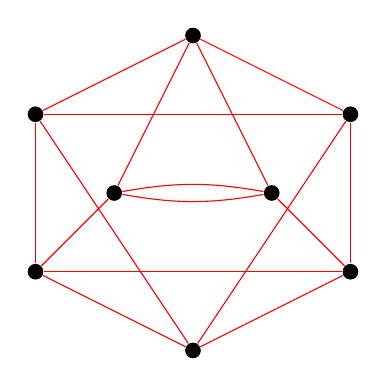
\begin{tikzpicture}
        \begin{scope}[every node/.style={fill,black,circle,inner sep=2pt}]
          \node at (0,0)  (1){};
          \node at (0,4) (20){};
          \node at (2,1)  (16z){};
          \node at (-2,1)  (81z){};
          \node at (-1,2) (77z){};
          \node at (1,2)  (20z){};
          \node at (-2,3)  (85z){};
          \node at (2,3)  (12z){};
        \end{scope}

        \begin{scope}[red]
          \path (1) edge (85z) edge (81z) edge (12z) edge (16z);
          \path (20) edge (85z) edge (77z) edge (20z) edge (12z);
          \path (81z) edge (85z) edge (77z) edge (16z);
          \path (85z) edge (12z);
          \path (12z) edge (16z);
          \path (16z) edge (20z);
          \path (20z) edge[bend right=10] (77z) edge[bend left=10] (77z);
        \end{scope}
      \end{tikzpicture}
      \small
      \emph{Figure:} $3$-isogeny graph on $\F_{97^2}$.
    \end{column}
  \end{columns}
\end{frame}

%%

\begin{frame}{Graphs lexicon}
  \begin{description}
  \item[Degree:] Number of (outgoing/ingoing) edges.
  \item[$k$-regular:] All vertices have degree $k$.
  \item[Connected:] There is a path between any two vertices.
  \item[Distance:] The length of the shortest path between two vertices.
  \item[Diamater:] The longest distance between two vertices.
  \item[$\lambda_1\ge\cdots\ge\lambda_n$:] The (ordered) eigenvalues
    of the adjacency matrix.
  \end{description}
\end{frame}

%%

\begin{frame}{Expander graphs}
  \begin{block}{Proposition}
    If $G$ is a $k$-regular graph, its largest and smallest
    eigenvalues satisfy
    \[k = \lambda_1 \ge \lambda_n \ge -k.\]
  \end{block}
  
  \begin{block}{Expander families}
    An infinite family of connected $k$-regular graphs on $n$ vertices
    is an \emph{expander family} if there exists an $\epsilon>0$ such
    that all \emph{non-trivial} eigenvalues satisfy
    $|\lambda| \le (1-\epsilon)k$ for $n$ large enough.
  \end{block}
  
  \begin{itemize}
  \item Expander graphs have \emph{short diameter} ($O(\log n)$);
  \item Random walks \emph{mix rapidly} (after $O(\log n)$ steps,
    the induced distribution on the vertices is close to uniform).
  \end{itemize}
\end{frame}

%%

\begin{frame}{Expander graphs from isogenies}
  \begin{block}{Theorem (\cite{pizer1,pizer2})}
    Let $\ell$ be fixed. The family of graphs of \emph{supersingular}
    curves over $\F_{p^2}$ with $\ell$-isogenies, as $p\to\infty$, is
    an expander family\footnote{Even better, it has the Ramanujan
      property.}.
  \end{block}
  
  \begin{block}{Theorem (\cite{jao+miller+venkatesan09})}
    Let $\O\subset\Q(\sqrt{-D})$ be an order in a quadratic imaginary
    field. The graphs of all curves over $\F_q$ with \emph{complex
      multiplication by $\O$}, with isogenies of prime degree
    bounded\footnote{May contain traces of GRH.} by
    $(\log q)^{2+\delta}$, are expanders.
  \end{block}
\end{frame}



%%%%%%%%%%%%%%%%%%%%%%%%%%%%%%%%%%%%%%%%%%%%%%%%%%%%%%%%%%%%%%%%%%%%%%%%%%%%%
%%%%%%%%%%%%%%%%%%%%%%%%%%%%%%%%%%%%%%%%%%%%%%%%%%%%%%%%%%%%%%%%%%%%%%%%%%%%%

\section{Cryptography}

\begin{frame}
  \frametitle{Overview}
  \tableofcontents  
\end{frame}

%%

\begin{frame}{History of isogeny-based cryptography}
  \begin{description}
  \item[1996] Couveignes introduces the \emph{Hard Homogeneous
      Spaces (HHS)}. His work stays unpublished for 10 years.
  \item[2006] Rostovtsev \& Stolbunov independently rediscover
    Couveignes ideas, suggest isogeny-based Diffie--Hellman as a
    \emph{quantum-resistant} primitive.
  \item[2007] Charles, Goren \& Lauter propose supersingular
    $2$-isogeny graphs as a foundation for a ``provably secure'' hash
    function.
  \item[2011-2012] D., Jao \& Plût introduce \emph{SIDH}, an
    efficient post-quantum key exchange inspired by Couveignes,
    Rostovtsev, Stolbunov, Charles, Goren, Lauter.
  \item[2017] SIDH is submitted to the NIST competition (with the name
    \emph{SIKE}, only isogeny-based candidate).
  \item[2018] Castryck, Lange, Martindale, Panny \& Renes publish an
    efficient variant of HHS named \emph{CSIDH}.
  \item[2019] New isogeny protocols: Signatures, Verifiable Delay Functions, \dots
  \end{description}
\end{frame}

%%%%%%%%%%%%%%%%%%%%%%%%%%%%%%%%%%%%%%%
%%%%%%%%%%%%%%%%%%%%%%%%%%%%%%%%%%%%%%%

\subsection{Isogeny walks and Hash functions}

\begin{frame}{Computing Isogenies}
  \begin{block}{Vélu's formulas}
    \begin{description}
    \item[Input:] A subgroup \emph{$H⊂E$},
    \item[Output:] The isogeny \emph{$ϕ:E→E/H$}.
    \item[Complexity:] \emph{$O(ℓ)$} --- \cite{velu71}, \dots
    \item[Why?]
      \begin{itemize}
      \item Evaluate isogeny on points \emph{$P∈E$};
      \item Walk in \emph{isogeny graphs}.
      \end{itemize}
    \end{description}
  \end{block}

  \pause
  
  \begin{block}{Explicit Isogeny Problem}
    \begin{description}
    \item[Input:] Curve \emph{$E$}, (prime) integer \emph{$ℓ$}
    \item[Output:] All subgroups \emph{$H⊂E$} of order
      \emph{$ℓ$}.
    \item[Complexity:] \emph{$\tildO(ℓ^2)$} --- \cite{elkies92}
    \item[Why?]
      \begin{itemize}
      \item List all isogenies of given degree;
      \item Count points of elliptic curves;
      \item Compute endomorphism rings of elliptic curves;
      \item Walk in \emph{isogeny graphs}.
      \end{itemize}
    \end{description}
  \end{block}
\end{frame}

%%

\begin{frame}{Computing Isogenies}
  \begin{block}{Explicit Isogeny Problem (2)}
    \begin{description}
    \item[Input:] Curves \emph{$E,E'$}, isogenous of degree \emph{$ℓ$}.
    \item[Output:] The isogeny \emph{$ϕ:E→E'$} of degree \emph{$ℓ$}.
    \item[Complexity:] \emph{$O(ℓ^2)$} ---
      \cite{elkies92,couveignes96,lercier+sirvent08,df10,defeo2016explicit,lairez-vaccon}, \dots
    \item[Why?]
      \begin{itemize}
      \item Count points of elliptic curves.
      \end{itemize}
    \end{description}
  \end{block}

  \pause
  
  \begin{block}{Isogeny Walk Problem}
    \begin{description}
    \item[Input:] Isogenous curves \emph{$E,E'$}.
    \item[Output:] An isogeny \emph{$ϕ:E→E'$} of \emph{smooth} degree.
    \item[Complexity:] Generically hard --- \cite{GHS}, \dots
    \item[Why?]
      \begin{itemize}
      \item Cryptanalysis (ECC);
      \item Foundational problem for \alert{isogeny-based cryptography}.
      \end{itemize}
    \end{description}
  \end{block}
\end{frame}

%%

\begin{frame}
  \frametitle{Random walks and hash functions (circa 2006)}

  Any expander graph gives rise to a hash function.

  \begin{center}
    \begin{tikzpicture}
      \coordinate (last) at (0,0);
      \draw (last) node[anchor=east] {$v$};
      \foreach \i in {1,...,6} {
        \pgfmathparse{(-1)^\i}
        \let\sign\pgfmathresult
        \pgfmathparse{int(mod(\i+1,2))}
        \let\bit\pgfmathresult
        \pgfmathparse{int(mod(\i,2))}
        \let\nbit\pgfmathresult
        \draw[->] (last) -- (\i,\sign*0.1) node[blue,pos=0.5,yshift=\sign*0.2cm]{\small$\bit$};
        \draw[dashed,->] (last) -- (\i,-\sign*0.5) node[gray,pos=0.5,yshift=-\sign*0.2cm]{\small$\nbit$};
        \coordinate (last) at (\i,\sign*0.1);
      }
      \draw (last) node[anchor=west] {$v'$};

      \node[blue,anchor=west] at (7,0) {$H(010101)=v'$};
    \end{tikzpicture}
  \end{center}

  \begin{itemize}
  \item Fix a starting vertex \emph{$v$};
  \item The value to be hashed determines a random path to \emph{$v'$};
  \item \emph{$v'$} is the hash.
  \end{itemize}

  \begin{block}{\parencite{charles+lauter+goren09} hash function (CGL)}
    \begin{itemize}
    \item Use the expander graph of \alert{supersingular
        $2$-isogenies};
    \item $\left.\begin{aligned}
          \text{\alert{Collision resistance}}&\\
          \text{\alert{2nd preimage resistance}}&
        \end{aligned}\right\} =$ hardness of finding cycles in the graph;
    \item \alert{Preimage resistance} = hardness of finding a path
      from \emph{$v$} to \emph{$v'$}.
    \end{itemize}
  \end{block}
\end{frame}

%%

\begin{frame}{Hardness of CGL}
  \begin{block}{Finding cycles}
    \begin{itemize}
    \item Analogous to finding endomorphisms\dots
    \item \dots very bad idea to start from a curve with \emph{known
        endomorphism ring}!
    \item Translation algortihm: \emph{elements of $B_{p,∞}$} $\leftrightarrow$ \emph{isogeny loops}\\
      Doable in \emph{$\polylog(p)$}.\footcite{kohel2014quaternion,10.1007/978-3-319-78372-7_11}
    \end{itemize}
  \end{block}

  \vspace{-1mm}
  
  \begin{block}{Finding paths $E\to E'$}
    \begin{itemize}
    \item Analogous to finding \emph{connecting ideals} between two
      maximal orders \emph{$\O,\O'$} (i.e. a \emph{left ideal} $I⊂\O$
      that is a \emph{right ideal} of $\O'$).
    \item Poly-time equivalent to computing \emph{$\End(E)$} and
      \emph{$\End(E')$}.\footcite{10.1007/978-3-319-78372-7_11}
    \item Best known algorithm to compute $\End(E)$ takes
      \emph{$\poly(p)$}.\footcite{kohel,cervino04}
    \end{itemize}
  \end{block}
\end{frame}

%%

\begin{frame}{\cite{kohel2014quaternion} (KLPT)}
   \begin{block}{}
     \begin{description}
     \item[Input:]
       \begin{itemize}
       \item Maximal order $\O⊂B_{p,∞}$ and associated curve $E$,
       \item Left ideal $I⊂\O$.
       \end{itemize}
     \item[Output:]
       \begin{itemize}
       \item Maximal order $\O'⊂B_{p,∞}$ s.t. $I$ connects $\O$ to $\O'$,
       \item \emph{Equivalent} ideal $J$ (i.e., also connecting $\O$ to
         $\O'$)\\ of [smooth/power-smooth] norm.
       \item Isogeny walk associated to $J$.
       \end{itemize}
     \end{description}
   \end{block}

  \begin{itemize}
  \item \emph{Complexity:} $\polylog(p)$,
  \item \emph{Output size:} $\polylog(p)$,
  \item Useful for:
    \begin{itemize}
    \item ``Shortening'' isogeny walks (see VDFs),
    \item ``Reducing'' isogeny walks (see Signatures),
    \end{itemize}
    when these start from a \emph{curve with known endomorphism ring}!\\
    (think $j=0,1728$ and other curves with small CM discriminant)
  \end{itemize}
\end{frame}

%%

\begin{frame}{Sampling supersingular curves}
  How to sample:
  \begin{itemize}
  \item A supersingular curve $E/\F_p$?
  \item A supersingular curve $E/\F_{p^2}$?
  \end{itemize}

  \begin{block}{Random walks}
    \begin{itemize}
    \item \emph{Start} from a supersingular curve $E_0$ with
      \emph{small CM discriminant}\\
      (e.g.: $j=1728$),
    \item Do a \emph{random walk} $E_0→E$ until reaching the
      \emph{mixing bound}\\
      ($O(\log(p))$ steps).
    \end{itemize}
  \end{block}

  \emph{Problem:} the random walk \emph{reveals $\End(E)$} via the
  KLPT algorithm.

  \begin{block}{Open problem}
    \textit{Give an algorithm to sample (uniformly) random
      supersingular curves in a way that does not reveal the
      endomorphism ring.}
  \end{block}
\end{frame}

%%%%%%%%%%%%%%%%%%%%%%%%%%%%%%%%%%%%%%%
%%%%%%%%%%%%%%%%%%%%%%%%%%%%%%%%%%%%%%%

\subsection{Pairing verification and Verifiable Delay Functions}

\begin{frame}{\cite{boneh+lynn+shacham04} signatures (BLS)}
  \begin{block}{}
    \begin{description}
    \item[Setup:]
      \begin{itemize}
      \item Elliptic curve $E/\F_p$, s.t $N|\#E(\F_p)$ for a large prime $N$,
      \item (Weil) pairing $e_N:E[N]×E[N]\to\F_{p^k}$ for some
        small embedding degree $k$,
      \item A decomposition $E[N]=X_1 × X_2$, with $X_1=〈P〉$.
      \item A hash function $H:\{0,1\}^*→X_2$.
      \end{itemize}
    \item[Private key:] $s∈ℤ/Nℤ$.
    \item[Public key:] $sP$.
    \item[Sign:] $m ↦ sH(m)$.
    \item[Verifiy:] $e_N(P,sH(m)) = e_N(sP,H(m))$.
    \end{description}
  \end{block}

  \centering
  \begin{tikzpicture}[ampersand replacement=\&]
    \matrix(m)[matrix of math nodes,row sep=3em,column sep=4em]{
      X_1 × X_2 \& X_1 × X_2\\
      X_1 × X_2 \& \F_{p^k}\\
    };
    \draw[->]
    (m-1-1) edge node[above]{\small$[s]\times 1$} (m-1-2)
    (m-1-1) edge node[left]{\small$1\times [s]$} (m-2-1)
    (m-1-2) edge node[right]{\small$e_N$} (m-2-2)
    (m-2-1) edge node[below]{\small$e_N$} (m-2-2);
  \end{tikzpicture}
\end{frame}

%%

\begin{frame}{US patent 8,250,367\footcite{broker2012cryptographic}}
  \begin{block}{Signatures from isogenies + pairings}
    \begin{itemize}
    \item Replace the secret \emph{$[s]:E→E$} with an isogeny \emph{$ϕ:E→E'$};
    \item Define decompositions
      \begin{align*}
        E[N] = X_1 × X_2, \qquad E'[N] = Y_1 × Y_2,
      \end{align*}
      s.t. \emph{$ϕ(X_1) = Y_1$} and \emph{$ϕ(X_2) = Y_2$};
    \item Define a hash function \emph{$H:\{0,1\}^*→Y_2$}.
    \end{itemize}
  \end{block}
  
  \begin{columns}
    \begin{column}{0.6\textwidth}
      \centering
      \begin{tikzpicture}[ampersand replacement=\&]
        \matrix(m)[matrix of math nodes,row sep=3em,column sep=4em]{
          X_1 × Y_2 \& Y_1 × Y_2\\
          X_1 × X_2 \& \F_{p^k}\\
        };
        \draw[->]
        (m-1-1) edge node[above]{\small$ϕ\times 1$} (m-1-2)
        (m-1-1) edge node[left]{\small$1\times\hat{ϕ}$} (m-2-1)
        (m-1-2) edge node[right]{\small$e_N'$} (m-2-2)
        (m-2-1) edge node[below]{\small$e_N$} (m-2-2);
      \end{tikzpicture}
    \end{column}
    \begin{column}{0.4\textwidth}
      \begin{uncoverenv}<2->
        \centering
        Useless, but nice!
      \end{uncoverenv}
    \end{column}
  \end{columns}
\end{frame}

%%

\begin{frame}{Verifiable Delay Functions}
  A Verifiable Delay Function (VDF) is a function \emph{$f:X→Y$} s.t.:
  \begin{itemize}
  \item \emph{Evaluating} $f$ at random $x∈X$ is \emph{provably
      ``slow''} (e.g., $\poly(\#X)$),
  \item Given $x∈X$ and $y∈Y$,\\
    \emph{verifying} that $f(x)=y$ can be done \emph{``fast''} (e.g.,
    $\polylog(\#X)$).
  \end{itemize}

  \begin{block}{(non)-Example: time-lock puzzles}
    \begin{itemize}
    \item Take a \emph{trapdoor} group $G$ of (e.g., \emph{$G=ℤ/Nℤ$}
      with \emph{$N=pq$});
    \item Define $f:G\to G$ as \emph{$f(g) = g^{2^T}$}:
      \begin{itemize}
      \item Best algorithm if $p,q$ known: \emph{compute $g^{2^T \bmod φ(pq)}$}
        \hfill$\polylog(N)$
      \item Best algorithm if $p,q$ unknown: \emph{$T$ squarings}
        \hfill$O(T)$
      \end{itemize}
    \end{itemize}
  \end{block}

  \begin{center}
    However, in VDFs we want to let \emph{anyone} verify efficiently.
  \end{center}
\end{frame}

%%

\begin{frame}{VDFs from groups of unknown order}
  \begin{block}{Interactive verification protocol \parencite{Wesolowski}}
    \begin{enumerate}
    \item Verifier chooses a prime \emph{$ℓ$} in a set of \emph{small
        primes} $\mathcal{P}$;
    \item Prover computes \emph{$2^T=aℓ+b$}, sends \emph{$g^{2^T},g^a$} to
      verifier;
    \item Verifier computes \emph{$2^T=aℓ+b$}, checks that
      \[g^{2^T} = (g^a)^ℓg^b\]
    \end{enumerate}
    Can be made non-interactive via \emph{Fiat-Shamir}.
  \end{block}

  Candidate groups of \emph{unknown order}:
  \begin{itemize}
  \item RSA groups $ℤ/Nℤ$, needs \emph{trusted third party} to
    generate $N=pq$;
  \item \emph{Quadratic imaginary class groups} $\Cl(-D)$ for large
    random discriminants $-D<0$.
  \end{itemize}
\end{frame}

%%

\begin{frame}{VDFs from isogenies and pairings\footcite{cryptoeprint:2019:166}}
  \centering
  \begin{tikzpicture}[ampersand replacement=\&]
    \matrix(m)[matrix of math nodes,row sep=3em,column sep=4em]{
      X_1 × Y_2 \& Y_1 × Y_2\\
      X_1 × X_2 \& \F_{p^k}\\
    };
    \draw[->]
    (m-1-1) edge node[above]{\small$ϕ\times 1$} (m-1-2)
    (m-1-1) edge node[left]{\small$1\times\hat{ϕ}$} (m-2-1)
    (m-1-2) edge node[right]{\small$e_N'$} (m-2-2)
    (m-2-1) edge node[below]{\small$e_N$} (m-2-2);
  \end{tikzpicture}

  \begin{description}
  \item[Setup:]
    \begin{itemize}
    \item \emph{Supersingular} curve \emph{$E/\F_p$} with (Weil)
      pairing $e_N$;
    \item\emph{Public isogeny} $ϕ:E→E'$ of degree
      \emph{$2^T$};
    \item The dual isogeny $\hat{ϕ}:E'→E$;
    \item A generator \emph{$〈P〉=X_1⊂E[N]$}, compute \emph{$ϕ(P)$}.
    \end{itemize}
  \item[Evaluate:] On input a random \emph{$Q∈Y_2⊂E'[N]$}, compute
    \emph{$\hat{ϕ}(Q)$}.
  \item[Verify:] Check that \emph{$e_N(P,\hat{ϕ}(Q)) = e_N'(ϕ(P),Q)$}.
  \end{description}
\end{frame}

%%

\begin{frame}{Security}
  \begin{description}
  \item[Obvious attack:] Pairing inversion must be hard (not
    post-quantum).
  \item[Wanted:] No better way to evaluate $\hat{ϕ}:E'→E$ than
    \emph{composing $T$ degree $2$ isogenies}.
  \end{description}

  \begin{block}{Shortcuts}
    \begin{itemize}
    \item If we can find a \emph{shorter way} from $E$ to $E'$, we can
      evaluate $\hat{ϕ}$ \emph{faster}.
    \item Shortcuts are easy to compute:
      \begin{itemize}
      \item If the isogeny graph is small (excludes ordinary pairing
        friendly curves);
      \item If $\End(E)$ or $\End(E')$ is known (via KLPT).
      \end{itemize}
    \item \emph{Needed:} choose $E/\F_p$ in a way that does not reveal
      $\End(E)$;
    \item \emph{Only known solution:} let a \emph{trusted third party}
      generate $E$.
    \end{itemize}
  \end{block}
  
\end{frame}

%%%%%%%%%%%%%%%%%%%%%%%%%%%%%%%%%%%%%%%
%%%%%%%%%%%%%%%%%%%%%%%%%%%%%%%%%%%%%%%

\subsection{Key exchange}

\begin{frame}{Let's get back to Diffie-Hellman}
  \begin{center}
    \begin{tikzpicture}[domain=-2.4566:4,samples=100]
      \newcount\rotate
      \animate<1-6>
      \animatevalue<2-6>{\rotate}{0}{90}
      \begin{scope}[rotate=-\the\rotate]
        \draw plot (\x,{0.5*sqrt(\x*\x*\x-4*\x+5)});
        \draw plot (\x,{-0.5*sqrt(\x*\x*\x-4*\x+5)});
      \end{scope}
      
      \begin{uncoverenv}<1>
        \begin{scope}[yscale=1/2]
          \draw[thin,gray,-latex] (0,-7) -- (0,7);
          \draw[thin,gray,-latex] (-3,0) -- (4,0);
          
          \draw (-3,1) -- (4,8/3+3);
          \begin{scope}[every node/.style={draw,circle,inner sep=1pt,fill},cm={1,2/3,0,0,(0,3)}]
            \node at (-2.287980,0) {};
            \node at (-0.535051,0) {};
            \node at (3.267475,0) {};
          \end{scope}
          \begin{scope}[every node/.style={yshift=0.3cm},cm={1,2/3,0,0,(0,3)}]
            \node at (-2.287980,0) {$P$};
            \node at (-0.535051,0) {$Q$};
            \node at (3.267475,0) {$R$};
          \end{scope}
          \draw[dashed] (3.267475,3.267475*2/3+3) -- (3.267475,-3.267475*2/3-3) 
          node[draw,circle,inner sep=1pt,fill] {}
          node[xshift=-0.1cm,anchor=east] {$P+Q$};
        \end{scope}
      \end{uncoverenv}
    \end{tikzpicture}
  \end{center}
\end{frame}

%%

\begin{frame}{Elliptic curves}
  \transdissolve
  \centering
  \includegraphics[height=0.7\textheight]{ec-happy}

  \Large\bf I power 70\% of WWW traffic!
\end{frame}

%%

\begin{frame}{The Q Menace}
  \centering
  \includegraphics[height=0.7\textheight]{qc-color}
\end{frame}

%%

\begin{frame}{Post-quantum cryptographer?}
  \centering
  \includegraphics[height=0.7\textheight]{ec-broke}
\end{frame}

%%

\begin{frame}{Elliptic curves of the world, UNITE!}
  \centering
  \begin{tikzpicture}
    \foreach \x/\y in {0/-0.5,4/2,8/-1}{
      \node at (\x,\y) {\includegraphics[height=3cm]{ec-banderole}};
    }
    \foreach \x/\y in {1/3,4.5/-1,7/3}{
      \node at (\x,\y) {\includegraphics[height=3.5cm]{ec-sign}};
    }
    \color{teal!70!blue}\itshape\bfseries\comicneue
    \node[rotate=-3] at (5.9,3.6) {\parbox{0pt}{QUOUSQUE\\QUANTUM?}};
    \node[rotate=-3] at (3.6,-0.4) {\parbox{0pt}{QUANTUM\\SUFFICIT!}};
  \end{tikzpicture}
\end{frame}

%%

\begin{frame}{And so, they found a way around the Q...}
  \centering
  \begin{tikzpicture}
    \comicneue\itshape
    \node at (0,0) {\includegraphics[height=2.5cm]{qc-color}};
    
    \node(E0) at (-5,0) {\includegraphics[height=1cm]{ec-happy}};

    \uncover<2->{
      \node(EA) at (0,3.5) {\includegraphics[height=1cm]{ec-happy}};
      \node(EB) at (0,-3.5) {\includegraphics[height=1cm]{ec-happy}};
      \draw[->,decorate,decoration=snake] (E0) to (EA);
      \draw[->,decorate,decoration=snake] (E0) to (EB);
      \node[right=0.3cm of EA] {\bl{Public curve}};
      \node[right=0.3cm of EB] {\bl{Public curve}};
    }
    \uncover<3>{
      \node(ES) at (5,0) {\includegraphics[height=1cm]{ec-happy}};
      \draw[->,decorate,decoration=snake] (EA) to (ES);
      \draw[->,decorate,decoration=snake] (EB) to (ES);
      \node[below=1em of ES] {\rd{Shared secret}};
    }
  \end{tikzpicture}
\end{frame}

%%

\begin{frame}
  \frametitle{Expander graphs from groups}
  \begin{center}
    \begin{tikzpicture}
      \begin{scope}
        \def\crater{12}
        \def\jumpa{-8}
        \def\jumpb{9}
        \def\diam{3cm}

        \foreach \i in {1,...,\crater} {
          \uncover<2->{\draw[blue] (360/\crater*\i : \diam) to[bend right] (360/\crater*\i+360/\crater : \diam);}
          \uncover<3->{\draw[red] (360/\crater*\i : \diam) to[bend right] (360/\crater*\i+\jumpa*360/\crater : \diam);}
          \uncover<4->{\draw[green] (360/\crater*\i : \diam) to[bend right=50] (360/\crater*\i+\jumpb*360/\crater : \diam);}
        }
        \foreach \i in {1,...,\crater} {
          \pgfmathparse{int(mod(2^\i,13))}
          \let\exp\pgfmathresult
          \draw[fill] (360/\crater*\i: \diam) circle (2pt) +(360/\crater*\i: 0.4) node{$g^{\exp}$};
        }
      \end{scope}
      \begin{scope}[xshift=4cm]
        \draw (0,2.1) node[anchor=west] {\parbox{4cm}{
            Let \emph{$G=\langle g\rangle$} be a cyclic group of order \emph{$p$}.
            \uncover<5->{Let \emph{$S\subset(\Z/p\Z)^\times$} s.t. \emph{$S^{-1}\subset S$}.\\
              The \emph{Schreier graph} of \emph{$(S,G\setminus\{1\})$} is (usually) an expander.}}};
        \uncover<2->{\draw[blue] (0,0) -- (0.5,0) (0.5,0) node[anchor=west] {$x \mapsto x^{2}$};}
        \uncover<3->{\draw[red] (0,-1) -- (0.5,-1) (0.5,-1) node[anchor=west] {$x \mapsto x^{3}$};}
        \uncover<4->{\draw[green] (0,-2) -- (0.5,-2) (0.5,-2) node[anchor=west] {$x \mapsto x^{5}$};}
      \end{scope}
    \end{tikzpicture}
  \end{center}
\end{frame}

%% 

{
  \newcommand{\myedge}[3]{
    \draw[#3] (360/\crater*#1 : \diam) to[bend right] (360/\crater*#2 : \diam);
  }

\begin{frame}
  \frametitle{Key exchange from Schreier graphs}

  \begin{columns}
    \begin{column}{0.55\textwidth}
      \begin{tikzpicture}
        \begin{scope}
          \def\crater{12}
          \def\jumpa{-8}
          \def\jumpb{9}
          \def\diam{2.5cm}
          
          \foreach \i in {1,...,\crater} {
            \pgfmathparse{int(mod(2^\i,13))}
            \let\exp\pgfmathresult
            \draw[fill] (360/\crater*\i: \diam) circle (2pt);
          }
          \uncover<2,6->{
            % Alice 1
            \myedge{0}{1}{blue}\myedge{1}{5}{red}\myedge{5}{6}{blue}\myedge{6}{3}{green}
          }
          \uncover<3,5>{
            % Bob 1
            \begin{scope}[dashed,thick]
              \myedge{0}{4}{red}\myedge{4}{8}{red}\myedge{8}{5}{green}\myedge{5}{6}{blue}
            \end{scope}
          }
          \uncover<5>{
            % Alice 2
            \myedge{6}{7}{blue}\myedge{7}{11}{red}\myedge{11}{0}{blue}\myedge{0}{9}{green}
          }
          \uncover<6->{
            % Bob 2
            \begin{scope}[dashed,thick]
              \myedge{3}{7}{red}\myedge{7}{11}{red}\myedge{11}{8}{green}\myedge{8}{9}{blue}
            \end{scope}
          }

          \draw (0 : \diam + 0.4cm) node {$g$};
          \uncover<2->{\draw (360/\crater*3 : \diam + 0.4cm) node {$g_A$};}
          \uncover<3->{\draw (360/\crater*6 : \diam + 0.4cm) node {$g_B$};}
          \uncover<5->{\draw (360/\crater*9 : \diam + 0.4cm) node {$g_{BA}\uncover<6->{=g_{AB}}$};}
        \end{scope}
      \end{tikzpicture}  
    \end{column}    
    \begin{column}{0.45\textwidth}
      \begin{onlyenv}<-6>
        \textbf{Public parameters:}
        \begin{itemize}
        \item A group \emph{$G=\langle g\rangle$} of order \emph{$p$};
        \item A subset \emph{$S\subset(\Z/p\Z)^\times$}.
        \end{itemize}
        \begin{enumerate}
        \item<2-> \textbf{Alice} takes a \alert{secret} random walk
          \emph{$s_A:g\to g_A$} of length \emph{$O(\log p)$};
        \item<3-> \textbf{Bob} does the same;
        \item<4-> They publish \emph{$g_A$} and \emph{$g_B$};
        \item<5-> \textbf{Alice} repeats her secret walk \emph{$s_A$}
          starting from \emph{$g_B$}.
        \item<6-> \textbf{Bob} repeats his secret walk \emph{$s_B$}
          starting from \emph{$g_A$}.
        \end{enumerate}
      \end{onlyenv}
      \begin{onlyenv}<7->
        \textbf{Why does this work?}
        \begin{align*}
          g_A &= g^{\bl{2}\cdot\rd{3}\cdot\bl{2}\cdot\gr{5}},\\
          g_B &= g^{\rd{3^2}\cdot\gr{5}\cdot\bl{2}},\\
          g_{BA} &= g_{AB} = g^{\bl{2^3}\cdot\rd{3^3}\cdot\gr{5^2}};
        \end{align*}
        and $g_A,g_B,g_{AB}$ are uniformly distributed in $G$\dots

        \bigskip
        
        \begin{uncoverenv}<8->
          \dots Indeed, this is just a twisted presentation of the
          \alert{classical Diffie-Hellman protocol!}
        \end{uncoverenv}
      \end{onlyenv}
    \end{column}
  \end{columns}
\end{frame}
}

%%

\begin{frame}
  \frametitle{Key exchange in graphs of ordinary isogenies\footcite{Couv,R&S} (CRS)}
  
  \emph{Parameters:}
  \begin{itemize}
  \item \emph{$E/\F_p$} ordinary elliptic curve, with Frobenius endomorphism \emph{$\pi\in\O$}.
  \item (small) primes \bl{$\ell_1$},\rd{$\ell_2$},\dots
    such that $\left(\frac{D_\pi}{\ell_i}\right)=1$.
  \item elements
    \bl{$\frak f_1=(\ell_1,\pi-\lambda_1)$}, \rd{$\frak f_2=(\ell_2,\pi-\lambda_2)$},\dots in
    $\Cl(\O)$.
  \end{itemize}

  \emph{Secret data:} \emph{Random walks} $\a,\b\in\Cl(\O)$ in the
  isogeny graph.
  
  \begin{center}
    \begin{tikzpicture}
      \Large
      \node[matrix of math nodes, ampersand replacement=\&, column sep=0cm, row sep=1cm] (diagram) {
        \& |(1)| E \\
        |(a)| \a\ast E \& \& |(b)| \b\ast E\\
        \& |(ab)| \a\b\ast E = \b\a\ast E\\
      };
      \small
      \path[->] (1) edge node[auto,swap]{$\bl{\frak f_1^{a_1}}\rd{\frak f_2^{a_2}}\cdots=\a$} (a);
      \path[->] (1) edge node[auto]{$\b=\bl{\frak f_1^{b_1}}\rd{\frak f_2^{b_2}}\cdots$} (b);
      \path[->] (a) edge (ab);
      \path[->] (b) edge (ab);
    \end{tikzpicture}
  \end{center}
\end{frame}

%%

\begin{frame}{Computing the action of $\Cl(\O)$}
  \begin{description}
  \item[Input:] An ideal class $\frak a = \bl{\frak f_1^{a_1}}\rd{\frak f_2^{a_2}}\cdots$.
  \item[Output:] The elliptic curve \emph{$\frak a\ast E$}.
  \item[Algorithm:] Let \emph{$\frak f^n=(\ell,\pi-\lambda)^n$},
    repeat \emph{n} times:
    \begin{itemize}
    \item Use \textbf{Elkies' algorithm} to find all (two) curves
      isogenous to \emph{$E$} of degree \emph{$\ell$},
    \item Choose the one such that
      \emph{$\ker\phi\subset\ker(\pi-\lambda)$}.
    \end{itemize}
  \end{description}

  \begin{block}{Parameters size / performance}
    \begin{description}
    \item[Adversary goal:] Given \emph{$E, \frak a*E$}, find
      \emph{$\a$};
    \item[Graph size:] \alert{$\#\Cl(\O) \approx \sqrt{p}$};
    \item[Best (classical) attack:] Meet-in-the-middle / Random-walk
      in \alert{$\sqrt{\#\Cl(\O)}$};
    \item[For $2^{128}$ security:] choose \alert{$\log p \sim 512$};
    \item[Time to evaluate the isogeny
      action\footcite{10.1007/978-3-030-03332-3_14}:] Dozens of minutes!
    \end{description}
  \end{block}
\end{frame}

%%

\begin{frame}{Vélu to the rescue?}
  \begin{description}
  \item[Input:] An ideal class $\frak a = \bl{\frak f_1^{a_1}}\rd{\frak f_2^{a_2}}\cdots$.
  \item[Output:] The elliptic curve \emph{$\frak a\ast E$}.
  \item[Algorithm:] Let \emph{$\frak f^n=(\ell,\pi-\lambda)^n$}.  Why
    not:
    \begin{itemize}
    \item \textit{Presciently} find \emph{$H = E[\ell]\cap\ker(\pi-\lambda)$},
    \item Apply Vélu's formulas to \emph{$H$}.
    \end{itemize}
  \end{description}

  \begin{block}{Speeding up the class group action}
    \begin{description}
    \item[Problem:] $H$ must be in $E(\F_p)$ for Vélu's formulas to be
      efficient.
    \item[Idea\footcite{10.1007/978-3-030-03332-3_14}:] Force
      $\begin{cases}
        p = -1 &\mod\ell,\\
        \alert<2->{\lambda = 1} &\alert<2->{\mod\ell},
      \end{cases}$\\
      so that \alert{$E[\ell] = H \subset E(\F_p)$}.
    \item<2->[How to waste an internship:] Forcing $\lambda =$ Forcing
      $\#E =$ \alert{Very hard!}
    \item<3->[Time to evaluate the isogeny action:] Still 5 minutes!
    \end{description}
  \end{block}
\end{frame}

%%

\begin{frame}{Supersingular to the rescue!}
  For all supersingular curves defined over $\F_p$,
  \begin{equation*}
    \pi = \begin{pmatrix}\sqrt{-p}&0\\0&-\sqrt{-p}\end{pmatrix} \mod\ell
  \end{equation*}
      
  \begin{block}{CSIDH \textit{(pron.: Seaside)}}
    \begin{description}
    \item[Choose] \alert{$p = -1 \bmod\ell$} for many primes $\ell$;
    \item[Hence,] \alert{$\lambda = 1 \mod \ell$}. Win!
    \item[Performance:] Same security as CRS in less than
      50ms!\footcite{10.1007/978-3-030-03332-3_15}
    \end{description}
  \end{block}
\end{frame}

%%

\begin{frame}{Quantum security}

  \textbf{Fact:} Shor's algorithm \emph{does not apply} to Diffie-Hellman
  protocols from \emph{group actions}.

  \begin{block}{Subexponential attack\hfill\emph{$\exp(\sqrt{\log p\log\log p})$}}
    \begin{itemize}
    \item Reduction to the \emph{hidden shift problem} by evaluating
      the class group action in \emph{quantum
        supersposition}~\footcite{childs+jao+soukharev10} (subexpoential cost);
    \item Well known reduction from the hidden shift to the
      \emph{dihedral (non-abelian) hidden subgroup problem};
    \item Kuperberg's algorithm\footcite{Kup,regev04,Kuperberg2013}
      solves the dHSP with a subexponential number of class group
      evaluations.
    \item Recent
      work\footcite{cryptoeprint:2018:432,cryptoeprint:2018:537,biasse2018note,Jao-etal-kuperberg-2018,cryptoeprint:2018:1059}
      suggests that $2^{64}$-qbit security is achieved somewhere in
      $512 < \log p < 1024$.
    \end{itemize}
  \end{block}
\end{frame}

%%

\begin{frame}
  \frametitle{Key exchange with supersingular curves (2011)}
  
  \begin{description}
  \item[Good news:] there is no action of a commutative class group.
  \item[Bad news:] there is no action of a commutative class group.
  \item[Idea:] Let \bl{Alice} and \rd{Bob} walk in two
    \emph{different isogeny graphs} on the \emph{same vertex set}.
  \end{description}

  \begin{columns}
    \begin{column}{0.7\textwidth}
      \centering
      \begin{tikzpicture}[scale=1.4]
        \begin{scope}[every node/.style={fill,black,circle,inner sep=2pt}]
          \node at (0,0)  (1){};
          \node at (0,4) (20){};
          \node at (2,1)  (16z){};
          \node at (-2,1)  (81z){};
          \node at (-1,2) (77z){};
          \node at (1,2)  (20z){};
          \node at (-2,3)  (85z){};
          \node at (2,3)  (12z){};
        \end{scope}

        \begin{uncoverenv}<1,3>
          \begin{scope}[blue,every loop/.style={looseness=50}]
            \path (1) edge (20) edge (16z) edge (81z);
            \path (20) edge[loop left] (20) edge[loop right] (20);
            \path (16z) edge (81z) edge (77z);
            \path (81z) edge (20z);
            \path (77z) edge (20z) edge (85z);
            \path (20z) edge (12z);
            \path (12z) edge[bend right=10] (85z) edge[bend left=10] (85z);
          \end{scope}
        \end{uncoverenv}
        
        \begin{uncoverenv}<2->
          \begin{scope}[red]
            \path (1) edge (85z) edge (81z) edge (12z) edge (16z);
            \path (20) edge (85z) edge (77z) edge (20z) edge (12z);
            \path (81z) edge (85z) edge (77z) edge (16z);
            \path (85z) edge (12z);
            \path (12z) edge (16z);
            \path (16z) edge (20z);
            \path (20z) edge[bend right=10] (77z) edge[bend left=10] (77z);
          \end{scope}
        \end{uncoverenv}
      \end{tikzpicture}
    \end{column}
    \begin{column}{0.3\textwidth}
      \small
      \emph{Figure:} \bl{$2$}- and \rd{$3$}-isogeny graphs on $\F_{97^2}$.
    \end{column}
  \end{columns}
\end{frame}

%%

\begin{frame}
  \frametitle{Key exchange with supersingular curves (2011)}

  \begin{itemize}
  \item Fix small primes \bl{$\ell_A$}, \rd{$\ell_B$};
  \item \emph{No canonical labeling} of the \bl{$\ell_A$}- and
    \rd{$\ell_B$}-isogeny graphs; \emph{however\dots}
  \end{itemize}

  \begin{center}
    \bf
    Walk of length \bl{$e_A$}\\
    $=$\\
    Isogeny of degree \bl{$\ell_A^{e_A}$}\\
    $=$\\
    Kernel \bl{$\langle P\rangle\subset E[\ell_A^{e_A}]$}
  \end{center}
  
  \begin{center}
    \begin{tikzpicture}
      \begin{scope}
        \draw (0,1.2) node[anchor=east,blue] {$\ker\phi=〈P〉\subset E[\ell_A^{e_A}]$};
        \draw (0,0.4) node[anchor=east,red] {$\ker\psi=〈Q〉\subset E[\ell_B^{e_B}]$};
        \draw (0,-0.4) node[anchor=east,blue] {$\ker\phi' = 〈\rd{\psi}(P)〉$};
        \draw (0,-1.2) node[anchor=east,red] {$\ker\psi' = 〈\bl{\phi}(Q)〉$};
      \end{scope}
      \begin{scope}[xshift=4.5cm,coils/.style={-angle 90,decorate,decoration={coil,aspect=0,amplitude=1pt}}]
        \large
        \node[matrix of nodes, ampersand replacement=\&, column sep=3cm, row sep=1.5cm] (diagram) {
          |(E)| $E$ \& |(Es)| $E/〈\bl{P}〉$ \\
          |(Ep)| {$E/〈\rd{Q}〉$} \& |(Eps)| {$E/〈\bl{P},\rd{Q}〉$}\\
        };
        \path[->,blue] (E) edge[coils] node[auto] {$\phi$} (Es);
        \path[->,blue] (Ep) edge[coils] node[auto,swap] {$\phi'$} (Eps);
        \path[->,red] (E) edge[coils] node[auto,swap] {$\psi$} (Ep);
        \path[->,red] (Es) edge[coils] node[auto] {$\psi'$} (Eps);
      \end{scope}
    \end{tikzpicture}
  \end{center}
\end{frame}

%%

\begin{frame}
  \frametitle{Supersingular Isogeny
    Diffie-Hellman\footcite{jao+defeo2011,defeo+jao+plut12}}

  \vspace{-1cm}

  \begin{columns}
    \begin{column}{0.4\textwidth}
      \begin{block}{}
        \emph{Parameters:}
        \begin{itemize}
          \setlength{\itemsep}{1.5ex}
        \item Prime $p$ such that $p+1 = \bl{\ell_A^a}\rd{\ell_B^b}$;
        \item Supersingular curve \emph{$E\simeq (\Z/(p+1)\Z)^2$};
        \item \bl{$E[\ell_A^a] = \cyc{P_A,Q_A}$};
        \item \rd{$E[\ell_B^b] = \cyc{P_B,Q_B}$}.
        \end{itemize}

        \emph{Secret data:}
        \begin{itemize}
          \setlength{\itemsep}{1.5ex}
        \item \bl{$R_A = m_AP_A + n_AQ_A$},
        \item \rd{$R_B = m_BP_B + n_BQ_B$},
        \end{itemize}
      \end{block}
    \end{column}
    \begin{column}{0.58\textwidth}
      \begin{center}
        \begin{tikzpicture}[coils/.style={-angle 90,decorate,decoration={coil,aspect=0,amplitude=1pt}}]
          \large
          \node[matrix of nodes, ampersand replacement=\&, column sep=4mm, row sep=2cm] (diagram) {
            \& |(1)| $E$ \\
            |(a)| \parbox{1.5cm}{$E/\cyc{\bl{R_A}}$\\\uncover<2->{{\footnotesize $\bl{\phi(}\rd{P_B}\bl{)}\\\bl{\phi(}\rd{Q_B}\bl{)}$}}} \& \&
            |(b)| \parbox{1.5cm}{$E/\cyc{\rd{R_B}}$\\\uncover<2->{{\footnotesize $\rd{\psi(}\bl{P_A}\rd{)}\\\rd{\psi(}\bl{Q_A}\rd{)}$}}}\\
            \normalsize $\frac{E/\cyc{\bl{R_A}}}{\alert{\bl{\phi(}\rd{R_B}\bl{)}}} \simeq$ \&
            |(ab)|  $E/\cyc{\bl{R_A},\rd{R_B}}$ \&
            \normalsize $\simeq \frac{E/\cyc{\rd{R_B}}}{\alert{\rd{\psi(}\bl{R_A}\rd{)}}}$\\
          };
          \small
          \path[blue] (1) edge[coils] node[auto,swap](phia) {$\phi$} (a);
          \path[red] (1) edge[coils] node[auto](phib) {$\psi$} (b);
          \path[red] (a) edge[coils] node[auto,swap](psia){$\psi'$} (ab);
          \path[blue] (b) edge[coils] node[auto](psib){$\phi'$} (ab);
          \uncover<3>{\path[dashed,->] (phia) edge node[auto]{\footnotesize $\bl{\phi(}\rd{R_B}\bl{)}$} (psia);}
          \uncover<3>{\path[dashed,->] (phib) edge node[auto,swap]{\footnotesize $\rd{\psi(}\bl{R_A}\rd{)}$} (psib);}
        \end{tikzpicture}
      \end{center}  
    \end{column}
  \end{columns}
\end{frame}

% 20. timeline of ibc, I need a hero

\begin{frame}{From 10 minutes to 10ms in 20 years}
  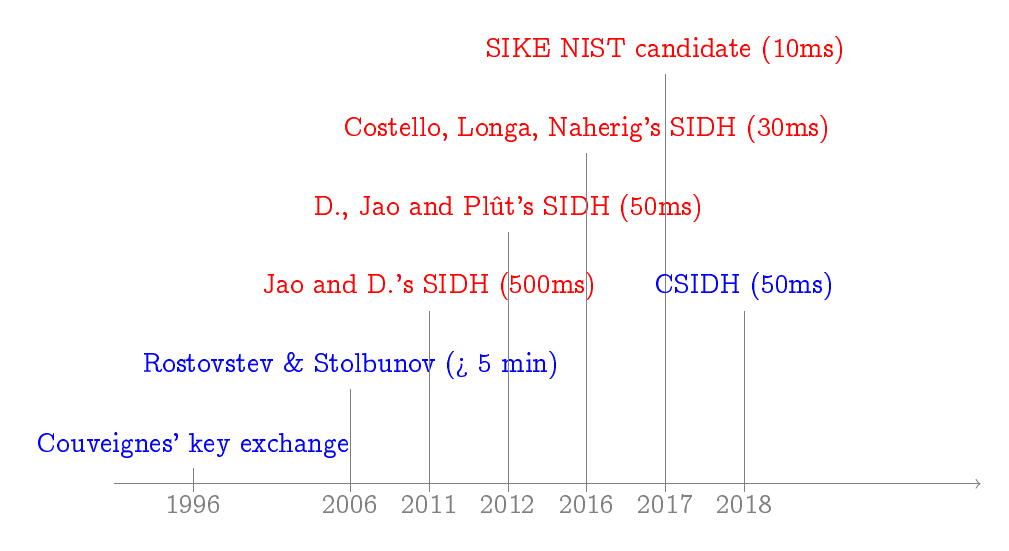
\begin{tikzpicture}[gray,every node/.style={anchor=south}]
    \draw[->] (0,0) -- (11,0);
    \uncover<1->{
      \node at (1,-0.5) {1996};
      \draw (1,-0.1) -- +(0,0.3) node[blue]{Couveignes' key exchange};
    }
    \uncover<2->{
      \node at (3,-0.5) {2006};
      \draw (3,-0.1) -- +(0,1.3) node[blue]{Rostovstev \& Stolbunov (> 5 min)};
    }
    \uncover<3->{
      \node at (4,-0.5) {2011};
      \draw (4,-0.1) -- +(0,2.3) node[red]{Jao and D.'s SIDH (500ms)};
    }
    \uncover<4->{
      \node at (5,-0.5) {2012};
      \draw (5,-0.1) -- +(0,3.3) node[red]{D., Jao and Plût's SIDH (50ms)};
    }
    \uncover<5->{
      \node at (6,-0.5) {2016};
      \draw (6,-0.1) -- +(0,4.3) node[red]{Costello, Longa, Naherig's SIDH (30ms)};
    }
    \uncover<6->{
      \node at (7,-0.5) {2017};
      \draw (7,-0.1) -- +(0,5.3) node[red]{SIKE NIST candidate (10ms)};
    }
    \uncover<7->{
      \node at (8,-0.5) {2018};
      \draw (8,-0.1) -- +(0,2.3) node[blue]{CSIDH (50ms)};
    }
  \end{tikzpicture}
\end{frame}


%%%%%%%%%%%%%%%%%%%%%%%%%%%%%%%%%%%%%%%
%%%%%%%%%%%%%%%%%%%%%%%%%%%%%%%%%%%%%%%

\subsection{Open Problems}

\begin{frame}{Open problems}
  From easier to harder:
  \begin{itemize}
  \item Give a convincing constant-time implementation of CSIDH.
  \item Find new isogeny-based primitives/protocols.
  \item Precisely asses the quantum security of CRS/CSIDH.
  \item Find an efficient post-quantum isogeny-based signature scheme.
  \item Exploit the extra information transmitted in SIDH/SIKE for
    cryptanalytic purposes.
  \item Sample supersingular curves without revealing endomorphism
    rings.
  \item Compute endomorphism rings of supersingular curves.
  \end{itemize}
\end{frame}

%%%%%%%%%%%%%%%%%%%%%%%%%%%%%%%%%%%%%%%
%%%%%%%%%%%%%%%%%%%%%%%%%%%%%%%%%%%%%%%

\begin{frame}
  \centering
  \begin{tikzpicture}
    \begin{scope}[xscale=1.2,black!60]
      \def\crater{7}
      \foreach \i in {1,...,\crater} {
        \draw[fill] (360/\crater*\i:3cm) circle (5pt);
        \draw (360/\crater*\i : 3cm) -- (360/\crater*\i+360/\crater : 3cm);
        \foreach \j in {-1,1} {
          \draw[fill] (360/\crater*\i : 3cm) -- (360/\crater*\i + \j*360/\crater/4 : 4cm) circle (3pt);
          \foreach \k in {-1,0,1} {
            \draw[fill] (360/\crater*\i + \j*360/\crater/4 : 4cm) --
            (360/\crater*\i + + \j*360/\crater/4 + \k*360/\crater/6 : 4.5cm) circle (1pt);
          }
        }
      }
    \end{scope}
    
    \draw (0,1) node{\Huge\bf Thank you};
    \draw (0,-0.6) node{\large\url{https://defeo.lu/}};
    \draw (0,-1.3) node{\large\includegraphics[height=0.9em]{twitter.png}~\href{https://twitter.com/luca_defeo}{@luca\_defeo}};
  \end{tikzpicture}
\end{frame}

%%

\begin{frame}[allowframebreaks]{References}
  \begin{block}{Surveys}
    \begin{itemize}
    \item \fullcite{Galbraith2018}.
    \item \fullcite{defeo2017isogenybased}.
    \item \fullcite{defeo-hdr}.
    \end{itemize}
  \end{block}

  \begin{block}{Elliptic curves and isogenies}
    \begin{itemize}
    \item \fullcite{silverman:elliptic}.
    \item \fullcite{milne1996elliptic}.
    \item \fullcite{blake+seroussi+smart}.
    \end{itemize}
  \end{block}

  \begin{block}{Isogeny graphs}
    \begin{itemize}
    \item \fullcite{kohel}.
    \item \fullcite{DelfsG16}.
    \item \fullcite{cryptoeprint:2018:593}.
    \end{itemize}
  \end{block}
  
  \begin{block}{Complex multiplication}
    \begin{itemize}
    \item \fullcite{silverman:advanced}.
    \item \fullcite{cox2011primes}.
    \end{itemize}
  \end{block}

  \begin{block}{Quaternion algebras}
    \begin{itemize}
    \item \fullcite{vigneras1980arithmetic}.
    \item \fullcite{Voight2018}.
    \end{itemize}
  \end{block}
\end{frame}

%%

\begin{frame}[allowframebreaks]
  \frametitle{Article citations}

  \defbibfilter{books}{\type{book} \or \type{booklet} \or \type{thesis}
    \or \type{report} \or \type{collection} \or \type{manual}
    \or \type{periodical} \or \type{proceedings}}
  \defbibfilter{articles}{\not \(\type{book} \or \type{booklet} \or \type{thesis}
    \or \type{report} \or \type{collection} \or \type{manual}
    \or \type{periodical} \or \type{proceedings}\)}

%  \beamertemplatebookbibitems
%  \printbibliography[filter=books]
  \beamertemplatearticlebibitems
  \printbibliography[filter=articles]
\end{frame}

\end{document}


% LocalWords:  Isogeny abelian isogenies hyperelliptic supersingular Frobenius
% LocalWords:  isogenous endomorphism


